

\documentclass[applsci,article,accept,pdftex,moreauthors]{Definitions/mdpi}
\usepackage[labelformat=simple]{subcaption}
\renewcommand\thesubfigure{\alph{subfigure}}
\DeclareCaptionLabelFormat{subcaptionlabel}{\normalfont(\textbf{#2}\normalfont)}
\captionsetup[subfigure]{labelformat=subcaptionlabel}

\firstpage{1} 
\makeatletter 
\setcounter{page}{\@firstpage} 
\makeatother
\pubvolume{1}
\issuenum{1}
\articlenumber{0}
\pubyear{2026}
\copyrightyear{2026}
\datereceived{ } 
\daterevised{ }
\dateaccepted{ } 
\datepublished{ } 
\hreflink{https://doi.org/}

\usepackage{caption}
\usepackage{subcaption}
\usepackage{booktabs}
\usepackage{longtable}
\usepackage{algorithm}
\usepackage{algpseudocode}
\renewcommand{\algorithmicrequire}{\textbf{Require:}}
\renewcommand{\algorithmicensure}{\textbf{Ensure:}}

\usetikzlibrary{shapes.misc, arrows.meta, positioning, fit, backgrounds}

\Title{A hybrid agent-based model of urban dengue transmission: city specific adaptation and validation in Santa Marta, Colombia}

\TitleCitation{Hybrid ABM of Dengue Transmission in Santa Marta}

\newcommand{\orcidauthorA}{0009-0005-6582-7986}
\newcommand{\orcidauthorB}{0009-0001-6438-7350} 
\newcommand{\orcidauthorC}{0009-0005-6845-2788} 
\newcommand{\orcidauthorD}{0009-0007-8227-373X}
\newcommand{\orcidauthorE}{0000-0003-4535-6521} 

\Author{Paula Escudero $^{1,\dagger, *}$\orcidA{}, Luisa F. Londoño $^{1, \dagger}$\orcidB{}, Sara M. Cano $^{1,\dagger}$\orcidD{} and Gabriel Parra $^{2,\dagger}$\orcidE{}}

\AuthorNames{Paula Escudero, Luisa F. Londoño, Sara M. Cano and Gabriel Parra}

\AuthorCitation{Escudero, P.; Londoño, L.; Cano, S.; Parra, G.}

\address{
$^{1}$ \quad Universidad EAFIT;[llondo61,pescuder,smcanom]@eafit.edu.co\\
$^{2}$ \quad Secretary of Health, District of Science, Technology, and Innovation of Medellín, Colombia; Gabriel.parrah@ucc.edu.co}

\corres{Correspondence: pescuder@eafit.edu}

\firstnote{These authors contributed equally to this work.}

 % \abstract{The \textit{Aedes aegypti} mosquito is a primary vector for diseases such as Dengue, Chikungunya, and Zika, which are increasing in prevalence globally. This study addresses the need to effectively model disease transmission dynamics in diverse urban settings by integrating a Hybrid Agent-Based Modeling Simulation (HABMS) approach with High-Performance Computing (HPC). Our model incorporates detailed factors such as geospatial, climate, and human aspects, providing a comprehensive and realistic simulation of disease dynamics despite the increased complexity and validation challenges. By integrating variables like temperature, human behavior, and geographic layout, our model allows the simulation of human movement patterns and contextual analysis within urban environments. It employs discrete-time equations for mosquito population modeling, enhancing computational efficiency and scalability. We tested the framework in the Colombian city of Santa Marta, demonstrating its adaptability to different urban settings. We calibrated the model's transmission parameters with surrogate-based Bayesian optimization and assessed their influence through a sensitivity analysis, with high-performance computing making these large sets of simulations feasible. The calibrated model reproduced the magnitude and the seasonal shape of the observed epidemic, and the late low tail of the season marks a clear direction for further refinement. Future work will add external introductions of infection and seasonal forcing, aiming to develop a robust tool that supports decision-making in mitigating vector-borne diseases in Colombia. This study contributes to vector-borne disease modeling, offering a powerful tool for public health interventions in varied urban environments.

\abstract{
Urban transmission of dengue and other \textit{Aedes aegypti}-borne diseases is shaped by the interaction of vector ecology, human mobility, climate, and spatial heterogeneity. Capturing these interactions in city-specific settings requires models that are detailed enough to represent local transmission processes, while remaining computationally feasible for calibration, validation, and sensitivity analysis. This study presents a Hybrid Agent-Based Modeling and Simulation (HABMS) approach, supported by High-Performance Computing (HPC), for simulating urban vector-borne disease transmission. Human residents are represented as mobile agents with stochastic infection dynamics, while mosquito populations are represented at the patch level through discrete-time equations. The model incorporates geospatial structure, temperature, land-use-based human movement, and local contextual information to represent transmission within urban environments.
The framework was applied to Santa Marta, Colombia, as a city-specific case study. Transmission parameters were calibrated using surrogate-based Bayesian optimization, and their influence was assessed through sensitivity analysis. High-performance computing made the large number of stochastic simulations required for calibration and sensitivity analysis feasible. The calibrated model reproduced the magnitude and main seasonal shape of the observed dengue epidemic, including the peak and early decline. However, the model did not fully reproduce the late low-incidence tail of the season, indicating the need to incorporate external introductions of infection and seasonal forcing in future versions. This study contributes an applied and computationally feasible hybrid simulation workflow for adapting, calibrating, and evaluating urban vector-borne disease models, with potential use in future decision-support analyses for dengue control in Colombia.
}

\keyword{Agent-based modeling and simulation; ABMS; HABMS; HPC; Dengue; Chikungunya; Zika; Vector-borne disease} 

\begin{document}

% \section{Introduction}

% \textit{Aedes aegypti} is the primary vector for dengue, chikungunya, and Zika, whose prevalence has risen markedly in recent years, affecting millions of people worldwide \cite{melo2024integrated}. Reports from the Pan American Health Organization (PAHO) and the World Health Organization (WHO) indicate that 2023 recorded approximately 4.6 million dengue cases in the Region of the Americas. By epidemiological week (EW)~12 of 2024, 3.6~million dengue cases had been reported, with 2{,}888 classified as severe (0.08\%) and 1{,}039 resulting in fatalities (0.029\%) \cite{ops2024}. This is more than a threefold increase compared with the same period in 2023. In Colombia, 69{,}837 cases were reported between EW~1--11 of 2024, a 262\% increase relative to the five-year average for the same period; the cumulative incidence at EW~11 was 136 per 100{,}000 population \cite{ops2024}. These figures fit a longer-term pattern: a systematic review reports that dengue has been hyperendemic in Colombia for years, with all four serotypes circulating and a persistent disease burden despite control efforts \cite{RodriguezMorales2024DengueColombia}.

% Local evidence from Santa Marta points to the environmental and demographic drivers behind this burden. A study of weekly dengue cases from 2009 to 2023 combined surveillance records with satellite derived measures of the urban environment, including the Normalized Difference Vegetation Index (NDVI), the Normalized Difference Water Index (NDWI), land surface temperature, precipitation, and population density \cite{MARTIN2026100164}. Dengue incidence in the city was associated with these environmental, climatic, and demographic conditions, and several of the associations acted with a lag of one to four weeks. This city specific signal motivates a spatially explicit simulation approach for Santa Marta, one that links local environmental conditions and human exposure to the places where transmission occurs.

% Transmission occurs via bites from infected female mosquitoes, and the burden falls disproportionately on economically disadvantaged populations, particularly in suburban areas \cite{melo2024integrated}. Risk is further shaped by climate, social conditions, and human behavior, including travel and daily routines \cite{uribe2023ccc}. Climate directly influences the distribution and abundance of mosquito vectors, while mobility patterns, outdoor activities, and adherence to preventive measures affect exposure to vectors and the likelihood of transmission. By accounting for these interconnected factors, public-health efforts can be tailored to target high-risk areas and populations, helping to mitigate the impact of vector-borne diseases on human health and well-being.

% Disease dynamics have traditionally been modeled with compartmental models such as the Susceptible--Infected--Recovered (SIR) and Susceptible--Exposed--Infected--Recovered (SEIR) formulations, which rely on differential equations. The SIR model partitions the population into susceptible (S), infected (I), and recovered (R) groups, while the SEIR model adds an exposed (E) compartment for individuals who are infected but not yet infectious. These models are widely used and often predictive, but they assume well-mixed, homogeneous populations and abstract away from individual heterogeneity and decision-making \cite{hunter2022validating}.

% When population heterogeneity, individual decision-making, and geospatial characteristics play a critical role, a more granular approach is required. Agent-based models provide exactly this granularity. An agent-based model is a computer simulation in which agents interact with one another and with their environment, capturing both individual behaviors and emergent phenomena at the system level \cite{antelmi2022experimenting}. Agent-based and hybrid approaches increase realism by embedding individuals in space, capturing where people live, work, commute, and interact, and linking those contacts to environmental drivers such as temperature \cite{antelmi2022experimenting,uribe2023ccc}. Incorporating explicit geospatial detail helps identify high-risk areas and supports the evaluation of operational levers, including vector control with pyriproxyfen stations placed in priority zones \cite{Ligsay2023Pyriproxyfen}. Despite these advances, applications that jointly integrate fine-scale urban geography, human decision-making, environmental forcing, and explicit control design remain uneven across distinct city contexts.

% Despite these advantages, agent-based modeling and simulation (ABMS) is inherently complex and often demands substantial computational resources and execution time. Several strategies mitigate these demands. Hybrid models combine ABMS with other techniques such as differential equations, high-performance implementations exploit parallel computing and optimized algorithms to accelerate execution, and discretizing the governing equations reduces computational overhead without compromising model fidelity. In particular, combining Hybrid Agent-Based Modeling and Simulation (HABMS) with differential equations and high-performance computing (HPC) provides a powerful approach for modeling vector-borne disease transmission in large populations, since HABMS captures the complex interactions that drive transmission while HPC delivers the scalability and efficiency required for large-scale scenario simulations.

% The literature consistently highlights the critical role of human behavior in shaping disease spread dynamics \cite{Topirceanu2024SpatialMobilityABM}; however, ABMS remains constrained by computational complexity and the impracticality of real-scale experiments \cite{Zhang2025ABMEpidemicsReview}. The use of HPC for vector-borne disease modeling is still relatively novel, and research on HPC models for \textit{Aedes aegypti} dynamics is scarce: although ABMS has been integrated into HPC frameworks, a full HABMS approach has yet to be realized. A related limitation concerns scalability and transferability, since existing studies provide limited evidence on how such models can be adapted across diverse urban settings.

% This study addresses these gaps by integrating a discrete-time HABMS approach into an HPC framework, with the primary objective of developing a scalable model that is readily adaptable to different city geographies and climates. Incorporating heterogeneous geospatial characteristics, such as temperature, geography, and human behavior, enhances the model's versatility and applicability. The study makes three main contributions: (i) a generic model capable of simulating vector-borne disease dynamics across diverse city geographies and climates; (ii) improvements in computational efficiency that support scalability and adaptability across urban environments; and (iii) a case study in Santa Marta, Colombia, a city particularly vulnerable to \textit{Aedes aegypti}-transmitted diseases owing to its climatic and geospatial conditions and its status as a tourism hub.

% This study is situated within agent-based modeling and simulation, particularly its application to spatially explicit urban epidemiology. Human agents are embedded in a geospatial representation of the city, where their daily movements determine exposure to local mosquito populations. Transmission is represented through a hybrid agent equation architecture that combines individual-level human dynamics with patch-level vector dynamics, while high-performance execution makes calibration and sensitivity analysis feasible at city scale. The contribution is therefore methodological and applied: it provides a workflow for adapting, running, calibrating, and evaluating a hybrid agent-based model for a public-health problem in an urban context, rather than introducing a new agent architecture or coordination paradigm.

% Although the model still requires further calibration and validation, it already enables the analysis of disease behavior across settings. Users can configure it for different cities by adjusting the geography and temperature inputs. The geography input, provided as a GeoJSON file, delineates the coordinates of the urban area, while the temperature input, provided as a CSV file, contains historical minimum, maximum, and mean temperatures over a year. Both datasets are available online from reliable sources.

% The remainder of this paper is organized as follows. Section~\ref{sec:relatedwork} reviews related work on HABMS and epidemiological modeling, with particular attention to vector-borne disease transmission and the use of HPC frameworks, and identifies the gaps that this study addresses. Section~\ref{sec:methods} then describes the modeling approach, its implementation in Repast HPC, the city-specific spatial adaptation, and the calibration and validation carried out for the Santa Marta case study.

\section{Introduction}

\textit{Aedes aegypti} is the primary vector for dengue, chikungunya, and Zika, diseases whose prevalence has risen markedly in recent years and now affects millions of people worldwide \cite{melo2024integrated}. Reports from the Pan American Health Organization (PAHO) and the World Health Organization (WHO) indicate that 2023 recorded approximately 4.6 million dengue cases in the Region of the Americas. By epidemiological week (EW)~12 of 2024, 3.6~million dengue cases had been reported, with 2{,}888 classified as severe (0.08\%) and 1{,}039 resulting in fatalities (0.029\%) \cite{ops2024}. This is more than a threefold increase compared with the same period in 2023. In Colombia, 69{,}837 cases were reported between EW~1--11 of 2024, a 262\% increase relative to the five-year average for the same period; the cumulative incidence at EW~11 was 136 per 100{,}000 population \cite{ops2024}. These figures fit a longer-term pattern: a systematic review reports that dengue has been hyperendemic in Colombia for years, with all four serotypes circulating and a persistent disease burden despite control efforts \cite{RodriguezMorales2024DengueColombia}.

Local evidence from Santa Marta points to the environmental and demographic drivers behind this burden. A study of weekly dengue cases from 2009 to 2023 combined surveillance records with satellite-derived measures of the urban environment, including the Normalized Difference Vegetation Index (NDVI), the Normalized Difference Water Index (NDWI), land surface temperature, precipitation, and population density \cite{MARTIN2026100164}. Dengue incidence in the city was associated with these environmental, climatic, and demographic conditions, and several of the associations acted with a lag of one to four weeks. This city-specific signal motivates a spatially explicit simulation approach for Santa Marta, one that links local environmental conditions and human exposure to the places where transmission actually occurs.

Transmission occurs via bites from infected female mosquitoes, and the burden falls disproportionately on economically disadvantaged populations, particularly in suburban areas \cite{melo2024integrated}. Risk is further shaped by climate, social conditions, and human behavior, including travel and daily routines \cite{uribe2023ccc}. Climate influences the distribution and abundance of mosquito vectors directly, while mobility patterns, outdoor activities, and adherence to preventive measures affect how much people are exposed to vectors and, with that, the likelihood of transmission. Accounting for these interconnected factors allows public-health efforts to be targeted toward high-risk areas and populations, which helps mitigate the impact of vector-borne diseases on health and well-being.

Disease dynamics have traditionally been modeled with compartmental formulations such as the Susceptible--Infected--Recovered (SIR) and Susceptible--Exposed--Infected--Recovered (SEIR) models, which rely on differential equations. The SIR model partitions the population into susceptible (S), infected (I), and recovered (R) groups, while the SEIR model adds an exposed (E) compartment for individuals who are infected but not yet infectious. These models are widely used and often predictive, but they assume well-mixed, homogeneous populations and leave out individual heterogeneity and decision-making \cite{hunter2022validating}.

When population heterogeneity, individual decision-making, and geospatial characteristics play a critical role, a more granular approach is needed. Agent-based models offer that granularity: an agent-based model is a computer simulation in which agents interact with one another and with their environment, capturing both individual behaviors and the patterns that emerge from them at the system level \cite{antelmi2022experimenting}. This study is situated within that tradition, particularly its application to spatially explicit urban epidemiology. Human agents are embedded in a geospatial representation of the city, their daily movements determine exposure to local mosquito populations, and those contacts are linked to environmental drivers such as temperature \cite{antelmi2022experimenting,uribe2023ccc}. Adding explicit geospatial detail also helps identify high-risk areas and supports the evaluation of operational levers, such as vector control with pyriproxyfen stations placed in priority zones \cite{Ligsay2023Pyriproxyfen}. Even so, applications that bring together fine-scale urban geography, human decision-making, environmental forcing, and explicit control design in one model remain uneven across different city contexts.

Agent-based modeling and simulation (ABMS) is inherently complex, though, and often demands substantial computational resources and execution time. A few strategies help with that. Hybrid models combine ABMS with other techniques such as differential equations, high-performance implementations exploit parallel computing and optimized algorithms to accelerate execution, and discretizing the governing equations reduces computational overhead without giving up model fidelity. Combining Hybrid Agent-Based Modeling and Simulation (HABMS) with differential equations and high-performance computing (HPC) is a particularly useful combination for modeling vector-borne disease transmission in large populations: HABMS captures the interactions that drive transmission, while HPC provides the scalability needed to run large sets of scenario simulations.

The literature consistently points to human behavior as a key driver of disease spread \cite{Topirceanu2024SpatialMobilityABM}, but ABMS remains constrained by computational complexity and by how impractical real-scale experiments are \cite{Zhang2025ABMEpidemicsReview}. The use of HPC for vector-borne disease modeling is still relatively new, and research on HPC models for \textit{Aedes aegypti} dynamics is scarce: although ABMS has been integrated into HPC frameworks, fewer studies combine hybrid human--vector model structure, city-specific geospatial adaptation, calibration, validation, and sensitivity analysis within a single applied workflow. A related gap concerns scalability and transferability, since existing studies offer limited evidence on how such models can be adapted across different urban settings.

This study addresses these gaps by integrating a discrete-time HABMS approach into an HPC framework, with the aim of building a model that is readily adaptable to different city geographies and climates. Incorporating heterogeneous geospatial characteristics, such as temperature, geography, and human behavior, supports that versatility. The study makes three main contributions: (i) a model architecture designed to be adaptable to different city geographies and climates, demonstrated here through its application to a new urban context; (ii) improvements in computational efficiency that support scalability and adaptability across urban environments; and (iii) a case study in Santa Marta, Colombia, a city particularly vulnerable to \textit{Aedes aegypti}-transmitted diseases owing to its climatic and geospatial conditions and its status as a tourism hub.

The contribution is therefore methodological and applied. Transmission is represented through a hybrid agent-equation architecture that combines individual-level human dynamics with patch-level vector dynamics, and high-performance execution makes calibration and sensitivity analysis feasible at city scale. What this study offers is a workflow for adapting, running, calibrating, and evaluating a hybrid agent-based model for a public-health problem in an urban setting, not a new agent architecture or coordination paradigm.

% Although the model still requires further calibration and validation, it already enables the analysis of disease behavior across different settings. Users can configure it for other cities by adjusting the geography and temperature inputs. The geography input, provided as a GeoJSON file, delineates the coordinates of the urban area, while the temperature input, provided as a CSV file, contains historical minimum, maximum, and mean temperatures over a year. Both datasets are available online from reliable sources.
The model is designed to be configured for other urban settings by updating the city-dependent inputs, including the urban geography and temperature series. In this study, the workflow is demonstrated for Santa Marta, where the model is adapted, calibrated, and evaluated using local surveillance and contextual data. The geography input is provided as a GeoJSON file that delineates the urban area, while the temperature input is provided as a CSV file containing historical minimum, maximum, and mean temperatures over one year. This separation between the core transmission model and the city-specific inputs supports future applications in other urban contexts when comparable data are available.

The remainder of this paper is organized as follows. Section~\ref{sec:relatedwork} reviews related work on HABMS and epidemiological modeling, with particular attention to vector-borne disease transmission and the use of HPC frameworks, and identifies the gaps that this study addresses. Section~\ref{sec:methods} then describes the modeling approach, its implementation in Repast HPC, the city-specific spatial adaptation, and the calibration and validation carried out for the Santa Marta case study.
\section{Related Work}
\label{sec:relatedwork}

Assumptions about spatial heterogeneity and connectivity are foundational in mosquito-borne disease models because they determine how infections propagate across urban space. In a systematic review, \cite{Lee2021SpatialConnectivityReview} show that spatial connectivity is operationalized through a wide range of assumptions, from simple distance kernels to explicit movement and place-based interactions, and argue that these choices are often insufficiently justified with local evidence, limiting transferability across cities. As a concrete example, \cite{Topirceanu2024SpatialMobilityABM} use a spatial agent-based model to show how different human mobility patterns shape the size and timing of urban epidemic outbreaks, which illustrates why connectivity assumptions deserve careful justification. Consequently, although spatially explicit dengue models are increasingly common, the literature provides comparatively fewer \emph{reproducible} workflows for adapting an existing hybrid agent-based model (HABM) to a new urban context using open geospatial data, explicit place layers, and locally defensible connectivity and mobility structures. This gap is especially important when the goal is not to propose a new modeling framework, but rather to deploy and validate an established HABM in a distinct city with different land-use patterns and exposure opportunities.

In parallel, vector ecological structure and parameter heterogeneity motivate careful localization of mosquito submodels before policy-oriented inference. For instance, \cite{Cruz2023StochasticAedesLifeCycle} propose a stochastic life-cycle and dengue transmission model that emphasizes how explicit stage structure can alter outbreak timing and intervention effects, and \cite{Pascoe2025AedesLifeCycleABM} model the full \textit{Aedes aegypti} life cycle with an agent-based approach, showing that representing each developmental stage changes the predicted vector population. Moreover, locality-specific empirical studies indicate that key \textit{Aedes aegypti} life-history traits may differ across populations; in particular, \cite{ArevaloCortes2022InsectsColombiaAedes} quantify differences in hatching, development, oviposition, and longevity among Colombian populations, supporting the premise that demographic parameters should not be treated as universal constants. Therefore, for urban dengue applications, a recurrent methodological need is to combine entomological realism with locally plausible parameter ranges and structural checks.

These modeling requirements interact directly with computational feasibility. Spatially explicit HABMs typically require large sets of stochastic runs to characterize variability and to perform uncertainty and sensitivity analyses at relevant spatial and temporal scales. In this regard, \cite{cyberCIS} demonstrates how high-performance computing can enable spatiotemporal uncertainty and sensitivity analysis in a dengue ABM, quantifying how parameter influence varies across clustered regions and over time. A recent review by \cite{Zhang2025ABMEpidemicsReview} likewise highlights computational scaling and calibration as central, still-open challenges for agent-based models of epidemics. Nevertheless, many studies treat computational scaling, uncertainty quantification, and calibration as separable tasks, whereas policy-relevant use often requires integrating them into a single workflow that remains feasible on fine-grained urban grids. Therefore, performance-aware implementations (e.g., parallel scheduling, efficient data structures, and output pipelines) become methodological enablers rather than purely technical details.

Beyond computation, the credibility of ABM-based decision support depends on systematic verification and validation practices. A recent overview by \cite{validationOverview} emphasizes that ABM validation lacks a universal standard, in part because model complexity and data limitations can render conventional statistical tests inadequate. Complementarily, \cite{credibilityPaper} argue that confidence in model-based decision support depends on verification, validation, and accreditation, even though public-sector accreditation procedures are often underdeveloped. These observations underscore that, for applied HABMs, methodological contributions frequently lie in how models are adapted, checked, and evaluated against fit-for-purpose criteria, rather than in proposing new model classes.

Within this credibility context, calibration remains a fundamental yet challenging stage. Calibration aims to adjust parameters so that simulations reproduce empirical patterns \cite{emo}. However, ABMs are typically non-linear and stochastic, which rules out closed-form likelihoods and complicates standard estimation \cite{Fagiolo2019}. Furthermore, the discrete-time structure of many ABMs encourages simulation-based approaches and intensifies computational demands \cite{fagiolo2007}. Classical approaches such as the method of simulated moments align simulated and observed moments but can be sensitive to moment selection and require substantial Monte Carlo sampling \cite{chenchang,Fagiolo2019}. Likewise, evolutionary multi-objective optimization methods can improve fit across multiple targets but remain stochastic and may degrade in performance as dimensionality increases \cite{emo}. To reduce simulation burden, mean-field approximations \cite{mean_field_method}, regression-based calibration \cite{regression}, and machine-learning surrogates \cite{machinelear} have been proposed. Nonetheless, these methods introduce additional assumptions, such as linear mappings or informative priors, and may trade accuracy for speed.

More recent inference frameworks directly target the computational bottleneck and the need for principled calibration diagnostics. \cite{OGara2025HistoryMatching} show that history matching combined with heteroskedastic Gaussian process emulation and likelihood-free inference can substantially increase the feasibility of calibrating high-resolution, stochastic ABMs, thereby expanding the space of policy analyses that can be performed under uncertainty. In addition, \cite{Horii2024SBCVerification} advocate simulation-based calibration (SBC) to verify whether a calibration procedure is statistically well-calibrated for stochastic disease ABMs, clarifying the distinction between \emph{calibration verification} and external, data-based validation. These developments support workflows in which repeated stochastic simulation is used not only for point fitting but also for probabilistic assessment, including uncertainty quantification and sensitivity analysis.

\section{Methods}
\label{sec:methods}

We adopted a staged methodological workflow that progressed from conceptualization and implementation to city-specific configuration, calibration, and validation. The study builds on two Colombian case studies with different urban contexts. Bello served as the development and feasibility phase, and Santa Marta is the primary case study presented in this paper.

\subsection{Staged modeling approach}
\label{sec:pipeline}

The methodology follows a five-stage workflow designed for the reproducible city-specific adaptation of a hybrid agent-based model for vector-borne disease transmission (Figure~\ref{fig:pipeline}). The workflow integrates spatial adaptation, expert-informed biological parameterization, high-performance execution, simulation-based calibration, and pattern-oriented validation into a single end-to-end process.

Stages~1 and~2 correspond to prior development work carried out for Bello and reported in detail elsewhere~\cite{escudero2023hybrid,uribe2023ccc}. Stage~1 produced the conceptual model under the ODD protocol~\cite{grimm2010odd}, defining the SEIR human agent structure, the discrete-time SEI mosquito dynamics, and the spatial grid topology. Stage~2 evaluated three agent-based frameworks and established Repast HPC~2.3.1 as the platform of choice based on parallelization support, memory efficiency, and scalability~\cite{uribe2023ccc}.

Stages~3 through~5 are the new contributions of this paper, applied to Santa Marta. Stage~3 adapts the existing model to Santa Marta by instantiating a GIS-based gridded topology, defining the urban mask and land-use zoning, and delineating sentinel neighborhoods. Stage~4 performs surrogate-based simulation calibration of the initial seed and the transmission parameters against weekly dengue surveillance data, corrected for under-reporting. Stage~5 validates the calibrated model through prediction-band coverage, shape-oriented temporal correlation, expert epidemiological review, and sensitivity analysis.

\begin{figure}[H]
\centering
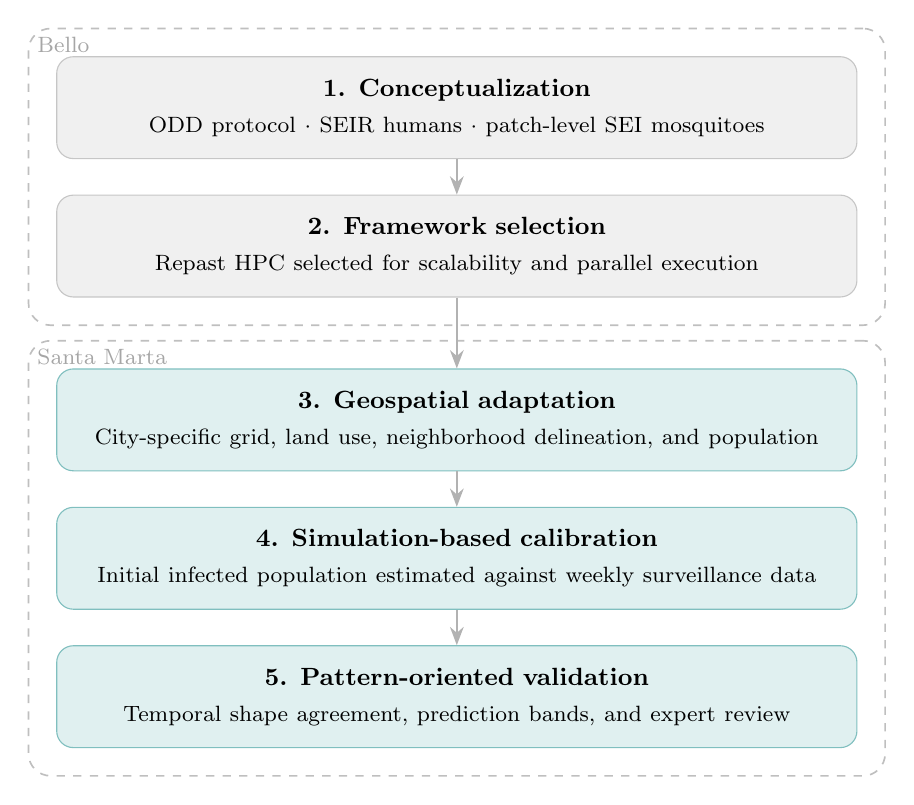
\begin{tikzpicture}[
  every node/.style = {font=\small},
  stage/.style = {
    rounded corners=6pt,
    minimum width=10cm,
    minimum height=1.1cm,
    align=center,
    text width=9.6cm,
    inner sep=8pt
  },
  gray stage/.style = {
    stage,
    fill=gray!12,
    draw=gray!45,
    line width=0.4pt
  },
  teal stage/.style = {
    stage,
    fill=teal!12,
    draw=teal!50,
    line width=0.4pt
  },
  band/.style = {
    rounded corners=8pt,
    draw=gray!50,
    line width=0.6pt,
    dashed,
    inner sep=10pt
  },
  arrow/.style = {
    -Stealth,
    gray!60,
    line width=0.8pt
  }
]

\node[gray stage] (s1) {%
  \textbf{1. Conceptualization}\\[2pt]
  {\footnotesize ODD protocol $\cdot$ SEIR humans $\cdot$ patch-level SEI mosquitoes}
};

\node[gray stage, below=0.45cm of s1] (s2) {%
  \textbf{2. Framework selection}\\[2pt]
  {\footnotesize Repast HPC selected for scalability and parallel execution}
};

\node[teal stage, below=0.9cm of s2] (s3) {%
  \textbf{3. Geospatial adaptation}\\[2pt]
  {\footnotesize City-specific grid, land use, neighborhood delineation, and population}
};

\node[teal stage, below=0.45cm of s3] (s4) {%
  \textbf{4. Simulation-based calibration}\\[2pt]
  {\footnotesize Initial infected population estimated against weekly surveillance data}
};

\node[teal stage, below=0.45cm of s4] (s5) {%
  \textbf{5. Pattern-oriented validation}\\[2pt]
  {\footnotesize Temporal shape agreement, prediction bands, and expert review}
};

\draw[arrow] (s1.south) -- (s2.north);
\draw[arrow] (s2.south) -- (s3.north);
\draw[arrow] (s3.south) -- (s4.north);
\draw[arrow] (s4.south) -- (s5.north);

\begin{scope}[on background layer]
  \node[band, fit=(s1)(s2), label={[font=\footnotesize\color{gray!70}, anchor=north west]north west:Bello}] {};
\end{scope}

\begin{scope}[on background layer]
  \node[band, fit=(s3)(s4)(s5), label={[font=\footnotesize\color{gray!70}, anchor=north west]north west:Santa Marta}] {};
\end{scope}

\end{tikzpicture}
\caption{Modelling workflow. Stages~1--2 were developed for Bello~\protect\cite{escudero2023hybrid,uribe2023ccc}. Stages~3--5 are new contributions presented in this paper for Santa Marta.}
\label{fig:pipeline}
\end{figure}

\subsection{Model architecture}
\label{sec:architecture}

The HABM represents a hybrid approach in which human agents follow individual-level stochastic dynamics while mosquito populations evolve as patch-level compartmental systems governed by discrete-time equations. This section describes the core architectural components shared across both case studies. Full implementation details for the Bello prototype are available in~\cite{escudero2023hybrid,uribe2023ccc}; here we present only the formulations required for the Santa Marta adaptation.

\subsubsection{Disease natural history}
\label{sec:natural_history}

The model captures dengue transmission by the female \textit{Aedes aegypti} mosquito~\cite{kakarla2019temperature}. After a blood meal, the virus infects the mosquito midgut and spreads to the salivary glands before onward transmission is possible~\cite{escudero2023hybrid}. Climate conditions modulate mosquito development rates and viral incubation times~\cite{goindin2015parity,Leung2020}; human-to-human transmission is not modeled~\cite{caminade2017global}.

Humans progress through four infection states, namely susceptible~(S), exposed~(E), infected~(I), and recovered~(R). The transition from exposed to infected occurs once the intrinsic incubation period (IIP) elapses, and recovery confers immunity over the one-year simulation horizon. Mosquitoes pass through three states, namely susceptible, exposed, and infected. They do not recover because their lifespan is approximately two to three weeks~\cite{goindin2015parity,scheidegger2017agent}. Table~\ref{table:distributions} lists the stochastic distributions used for the IIP and the infectious period. The framework supports the three arboviruses in Table~\ref{table:distributions}, and the present case study demonstrates the dengue configuration, with the Zika and chikungunya parameters provided to support future application of the same workflow to those diseases.

\begin{table}[H]
\caption{Stochastic distributions for intrinsic incubation time $t_{inc,h}$ and infectious period $t_{inf,h}$ by virus.}
\label{table:distributions}
\begin{tabularx}{\textwidth}{>{\centering\arraybackslash}p{2.5cm}
                              >{\centering\arraybackslash}p{5.5cm}
                              >{\centering\arraybackslash}p{5cm}}
\toprule
\textbf{Virus} & \textbf{Incubation time $t_{inc,h}$} & \textbf{Infectious period $t_{inf,h}$} \\
\midrule
Zika        & Weibull$(\alpha=2.69,\;\beta=6.70)$~\cite{Krow-Lucal2017}         & Normal$(\mu=6,\;\sigma=1)$~\cite{PMID:29617955} \\
Dengue      & Gamma$(\alpha=5.5,\;\beta=1.12)$~\cite{Chan2012}                  & Uniform$(a=2,\;b=7)$~\cite{Chan2012} \\
Chikungunya & Lognormal$(\mu=1.099,\;\sigma=0.139)$~\cite{Leung2020,manore2015eqs} & Uniform$(a=3,\;b=7)$~\cite{manore2015eqs} \\
\bottomrule
\end{tabularx}
\end{table}

\subsubsection{Spatial structure}
\label{sec:spatial}

The spatial environment is a two-dimensional grid of square patches covering the urban extent of the study city. Each patch is a static agent that stores local mosquito compartment counts (susceptible~$M_s$, infected~$M_i$) and the current temperature, and receives mobile human agents as they move during the day. Patches are assigned one of four land-use types, namely residential, study, work, or leisure, and these types guide the assignment of daily destinations to human agents. Only patches whose centroids fall within a preprocessed urban mask are activated, excluding water bodies and non-residential zones. State variables for humans and patches are listed in Tables~\ref{table:state_var_humans} and~\ref{table:state_var_patches}.

\begin{table}[H]
\centering
\caption{State variables for human agents.}
\label{table:state_var_humans}
\begin{tabularx}{\textwidth}{>{\bfseries}p{3.5cm} X}
\toprule
Variable & Description \\
\midrule
Infection state (SEIR) & Current compartment: susceptible, exposed, infected, or recovered. Changes at each movement event. \\
Time since successful bite & Days elapsed since the agent received an infectious bite and entered the exposed state; null if never bitten. \\
Time since infected & Days elapsed since the agent entered the infected state; null otherwise. \\
Home location & Coordinates of the residential patch assigned at initialization. \\
Age & Assigned at initialization from empirical age-band probabilities; constant over the simulation. Used to assign study or work destinations. \\
Activity list & Coordinates of two daily destinations (study/work and leisure), consistent with land-use zoning. \\
\bottomrule
\end{tabularx}
\end{table}

\begin{table}[H]
\centering
\caption{State variables for patches.}
\label{table:state_var_patches}
\begin{tabularx}{\textwidth}{>{\bfseries}p{3.5cm} X}
\toprule
Variable & Description \\
\midrule
$M_s$ & Number of susceptible adult mosquitoes. Updated three times per day. \\
$M_i$ & Number of infected adult mosquitoes. Updated three times per day. \\
Temperature & Daily temperature in \textdegree C, updated three times per day from the input climate series. \\
Land-use type & Residential (1), study (2), work (3), or leisure (4). Determines eligibility as a destination. \\
Neighborhood tag & Integer identifier for sentinel neighborhood membership; 0 if unassigned. \\
Emergence multiplier $\omega_i$ & Patch-level scalar applied to aquatic recruitment, informed by the House Index (Section~\ref{sec:hi_emergence}). Fixed at initialization. \\
\bottomrule
\end{tabularx}
\end{table}

\subsubsection{Human agent dynamics}
\label{sec:humans}

Each human agent represents one resident of the study city. Agents follow a daily activity schedule. They begin at their residential home patch, travel to a first destination (study or work, assigned by age), travel to a leisure destination, and return home at the end of the day. Infection risk is evaluated at each movement.

In patch~$k$, a susceptible human becomes exposed with probability
\begin{equation}
p_{SE,h}^{k} = 1 - \exp\!\left(-\lambda_h^{k}\right),
\quad
\lambda_h^{k} = b_h^{k}\,\beta_{mh}\left(\frac{M_i^{k}}{N_M^{k}}\right),
\quad
b_h^{k} = \frac{b^{k}}{N_H^{k}},
\label{eq:human_infection}
\end{equation}
where $M_i^{k}$ and $N_M^{k}$ are the infected and total mosquito counts in patch~$k$, $N_H^{k}$ is the number of human agents present, $\beta_{mh}$ is the mosquito-to-human transmission probability, and $b^k$ is the expected number of bites:
\begin{equation}
b^{k} =
\frac{\sigma_M N_M^{k}\;\sigma_H N_H^{k}}
     {\sigma_M N_M^{k} + \sigma_H N_H^{k}},
\label{eq:bites}
\end{equation}
with $\sigma_M$ and $\sigma_H$ the maximum bite rates per mosquito and per human per unit time. Transition from exposed to infected occurs when the time since the successful bite exceeds $t_{inc,h}$, drawn from the virus-specific distribution in Table~\ref{table:distributions}. Recovery occurs when the time since infection exceeds $t_{inf,h}$, drawn from the same table.

\subsubsection{Mosquito population dynamics}
\label{sec:mosquitoes}

Mosquito dynamics in each patch follow a discrete-time SEI system, updated three times per day to match human movement periods. Discrete equations are preferred because they align with the temporal resolution of public-health surveillance data and exhibit richer long-term dynamical behavior than continuous formulations when human and mosquito timescales differ substantially~\cite{cao2015discrete,li2019discrete}. Adapting the formulation of \citet{catano2022discrete}:
\begin{equation}
\begin{aligned}
M_{s}(t+1) &= M_{s}(t)\bigl(1-\beta_{hm}\Psi_{h}(t)\bigr)\bigl(1-\mu_{m}\bigr) + A(t), \\
M_{i}(t+1) &= M_{s}(t)\,\beta_{hm}\Psi_{h}(t)\bigl(1-\mu_{m}\bigr)
            + M_{i}(t)\bigl(1-\mu_{m}\bigr),
\end{aligned}
\label{eq:mosquito_dynamics}
\end{equation}
where $\beta_{hm}$ is the human-to-mosquito transmission probability, $\mu_m$ is the daily adult mortality rate, and
\begin{equation}
\Psi_{h}(t) = 1 -
\left[\frac{N_{h}(t) - H_{i}(t)}{N_{h}(t)}\right]^{z}
\label{eq:psi}
\end{equation}
is the human interaction probability, with $z$ the interaction parameter, $H_i(t)$ the number of infected humans, and $N_h(t)$ total humans in the patch. Aquatic recruitment follows a density-regulated Ricker expression:
\begin{equation}
A(t) = r\,N_m(t-2)\,\exp\!\left(1-\frac{N_m(t)}{C}\right),
\label{eq:ricker}
\end{equation}
where $r$ is the intrinsic reproduction rate, $C$ is the carrying capacity, and $N_m(t)=M_s(t)+M_i(t)$ is the total adult population. Adult mortality is linked to temperature through the polynomial response estimated by \citet{mortality_temp_estimate}:
\begin{equation}
\mu_m = P_m(T) = \sum_{i=0}^{4} b_i\,T^i,
\label{eq:mortality_temp}
\end{equation}
which captures the basin-shaped mortality profile of \textit{Aedes aegypti}, with lower values in the 15--30\,\textdegree C range and sharply increasing mortality at thermal extremes.

\subsubsection{High-performance execution and parallel experiments}
\label{sec:implementation}

The model is implemented in Repast HPC~2.3.1 with C++17 and MPI for distributed-memory parallelization~\cite{antelmi2022experimenting}. Two levels of parallelism support the study, and it is useful to keep them separate.

The first level acts inside a single simulation. Repast HPC divides the $135\times200$ grid into contiguous spatial blocks and assigns one block to each process. Every process then owns the human agents and mosquito patches in its block and advances their state on its own. Processes exchange information only about the agents and value layers that lie on the shared borders of their blocks. This division is safe for dengue, because the disease does not pass directly between humans. Infection on a given day is therefore local to a patch, so the partition does not distort the epidemic. When a human moves across a block boundary, the framework serializes that agent and transfers it to the neighboring process.

The second level acts across simulations. The heaviest cost of the study is not a single run but the large sets of runs needed for calibration and for sensitivity analysis. Each task evaluates many parameter combinations, and it repeats every combination over several stochastic replicates. These runs are independent of one another, so they can proceed at the same time. A driver launches many single-process simulations in parallel and chooses how many to run at once from the memory used by each run, which is about $0.1$~GB at the full scale of $10^5$ agents. Each run executes in its own working directory, with its own parameter file and its own output, so the concurrent runs do not interfere. After compiler optimization, one year of simulation at $10^5$ agents takes about half an hour on its own, and somewhat longer when many runs share the machine and compete for memory bandwidth. A calibration sweep or a sensitivity set of about one hundred runs therefore completes in a single overnight run on one multi-core workstation.

To keep the comparisons between configurations consistent, the runs share a common seed policy. The seed of run~$j$ is $s_{\text{base}}+j$, and the same replicate indices are reused across every configuration. This reduces Monte-Carlo variance in the paired comparisons. Daily temperature is drawn from a separate random stream, so temperature sampling does not interfere with the streams that drive infection and movement.

\subsection{City-specific adaptation for Santa Marta}
\label{sec:santamarta}

Building on the Bello prototype, the model was re-configured for Santa Marta by updating all city-dependent inputs while reusing the disease natural history and the HPC scaffolding from the prior phase. Santa Marta differs substantially from Bello in its coastal geography, tourism-driven economy, and epidemiological surveillance structure, which required specific adaptations in the spatial representation, mobility rules, and vector parameterization.

Santa Marta is a coastal Caribbean city that sits against the foothills of the Sierra Nevada. Its climate is tropical savanna, close to hot semi arid, with a marked dry season and a marked wet season \cite{MARTIN2026100164}. Long dry spells and an intermittent water supply lead many households to store water in elevated tanks, low tanks, jars, and other containers. These stored-water containers become important breeding sites for \textit{Aedes aegypti} in residential areas. This setting makes Santa Marta well suited as a case study for a spatially explicit model that links urban structure, human exposure, and mosquito dynamics within a single framework.

Santa Marta is represented as a regular grid of $135 \times 200$ cells covering 55.1~km$^2$, with each cell corresponding to approximately $45 \times 45$~m. Only cells whose centroids fall within the preprocessed urban mask are activated, yielding the effective simulation area. Land-use tags were derived from OpenStreetMap (OSM) data and converted to an empirical cumulative distribution to assign each active cell one of the four use categories. Because Santa Marta's coastal fringe concentrates tourist employment, a coastal bias was incorporated into the assignment of work cells to reflect the city's documented spatial pattern. This zoning supplied the substrate for daily mobility and mosquito-human contact opportunities.

A synthetic, down-scaled human population was initialized to preserve age structure while controlling runtime. Ages were sampled from empirical age-band probabilities and agents were placed on residential cells. Each agent was then assigned two daily destinations, one study or work location and one leisure location, by drawing from cells of the corresponding category. Agents placed on non-urban cells were excluded to prevent boundary artifacts. The case study used a population of $10^5$ agents, the scale at which the observed incidence is normalized to a rate per 100{,}000. This down-scaling preserved relative demographic and spatial patterns while keeping a one-year run to about half an hour after compiler optimization on the available hardware.

Vector dynamics were grounded in local entomology through an eighteen-day egg-to-adult development delay, stage-specific larval ($\sigma_L$) and pupal ($\sigma_P$) survival probabilities, and a realistic female emergence ratio~($f$). These values are consistent with life-history data reported for Colombian \textit{Aedes aegypti} populations~\cite{ArevaloCortes2022InsectsColombiaAedes}, and reflect the premise that demographic parameters should not be treated as universal constants when local estimates are available.

The same local evidence informs the structure of the model rather than its numerical inputs. The Santa Marta analysis linked dengue incidence to vegetation cover, land surface temperature, precipitation, water related conditions, and population density, with effects that varied in space and over time \cite{MARTIN2026100164}. This supports a central premise of the model, namely that transmission risk is spatially heterogeneous and depends on where people are located, where mosquito habitats persist, and how environmental conditions change through the year. The study estimated its associations with a generalized linear mixed model (GLMM), and those fitted coefficients are not used here as simulation parameters. The local analysis instead gives empirical support for the structural choices of the model: spatial heterogeneity in risk, local contact between humans and mosquitoes, temperature dependent mosquito dynamics, and delayed environmental processes that act over several weeks.

\subsection{Neighborhood delineation}
\label{sec:neighborhoods}

Sentinel neighborhoods were delineated as contiguous clusters of residential active cells on the model grid. They serve mainly to localize the HI-informed heterogeneity in vector recruitment described in Section~\ref{sec:hi_emergence} and to align the simulation with the project's operational focus on specific localities, rather than as independent units of sub-city epidemiological inference. Eight neighborhoods were delineated, namely Oasis, La~Quinina, Ondas del~Caribe, Pantano, 8~de~Diciembre, La~Coquera, San~Jacinto, and Nueva~Bethel.

Cluster growth proceeded via a breadth-first flood-fill (BFS) algorithm with ring-search seeding (Algorithm~\ref{alg:bfs}). The ring search ensured that the nominated seed coordinates could always be mapped to a valid residential active cell even when the nominal location fell on an inactive or non-residential patch. Once a valid seed was found, the BFS expanded contiguously by visiting orthogonal neighbors in layers, tagging each eligible cell with its neighborhood identifier and enqueuing its four neighbors. A cell was enqueued only if it was active, residential, and unassigned, guaranteeing disjointness between clusters. Growth terminated either when the target cell count was reached or when no further eligible residential cells were available.

Figure~\ref{fig:bfs_growth} illustrates the conceptual process. Starting from a seed cell (orange star), the algorithm expands outward to contiguous residential cells (dark blue) while excluding inactive cells and non-residential land uses. The arrows indicate the breadth-first expansion order, ensuring that neighborhoods grow contiguously until the target size or the available residential supply is reached.

\begin{figure}[H]
\centering
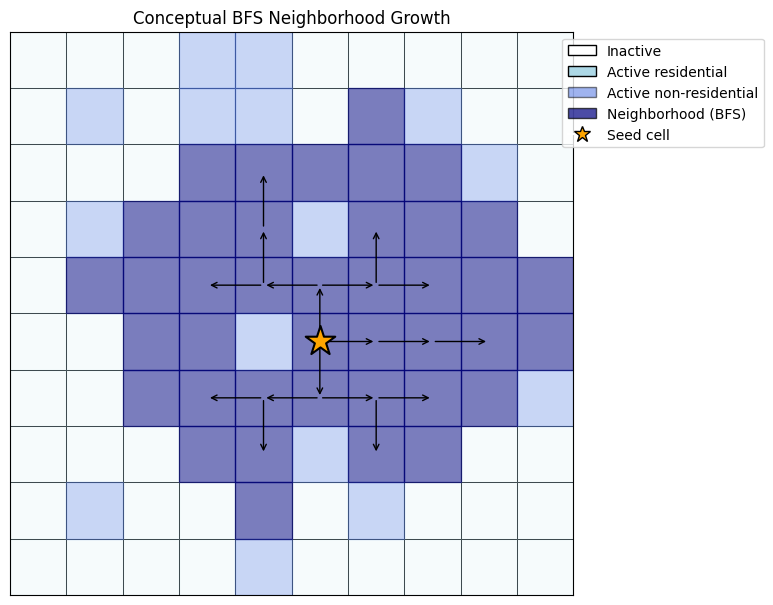
\includegraphics[width=0.5\textwidth]{Images/bfs.png}
\caption{Conceptual illustration of neighborhood clustering using a breadth-first flood-fill algorithm. The seed cell (orange star) initiates growth, and contiguous residential cells (dark blue) are iteratively added.}
\label{fig:bfs_growth}
\end{figure}

Target sizes were derived from reported neighborhood areas converted to equivalent cell counts using the estimated active-cell density. Post-assignment quality assurance verified three conditions, namely that all tagged cells were residential, that the clusters were pairwise disjoint, and that realized sizes fell within $\pm 5\%$ of their targets. Cases where residential supply was insufficient to meet the target were logged and interpreted in relation to the city's mixed land-use structure, as coastal and commercial areas naturally reduce the pool of contiguous residential cells in certain zones.

\begin{algorithm}[H]
\caption{BFS flood-fill with ring search for neighborhood delineation.}
\label{alg:bfs}
\begin{algorithmic}[1]
\Require Neighborhood ID $\mathit{nID}$, nominal seed $(c_x, c_y)$, target size $T$
\Require Layers: \textsc{Type} (1 = residential), \textsc{Neigh} (0 = unassigned), set \textsc{ActiveCells}
\Ensure Neighborhood tags written to \textsc{Neigh}; cell keys stored in the corresponding set
\State Initialize empty queue $Q$, set $\mathit{Visited} \leftarrow \emptyset$, counter $\mathit{filled} \leftarrow 0$
\For{radius $r = 0, \ldots, R_{\max}$} \Comment{Ring search for valid seed}
  \If{eligible cell $(x,y)$ found (active, residential, unassigned)}
    \State Mark $(x,y)$ visited; $\textsc{Enqueue}(Q,(x,y))$; \textbf{break}
  \EndIf
\EndFor
\If{$Q$ is empty} \Return (no residential seed found) \EndIf
\While{$Q \neq \emptyset$ \textbf{and} $\mathit{filled} < T$}
  \State $(x,y) \leftarrow \textsc{Dequeue}(Q)$
  \If{$\textsc{Neigh}[x,y] = 0$}
    \State $\textsc{Neigh}[x,y] \leftarrow \mathit{nID}$; record key; $\mathit{filled} \mathrel{+}= 1$
    \For{each 4-neighbor $(u,v) \in \{(x\pm1,y),(x,y\pm1)\}$}
      \If{$(u,v)$ in bounds, not visited, $(u,v) \in \textsc{ActiveCells}$, residential, unassigned}
        \State Mark $(u,v)$ visited; $\textsc{Enqueue}(Q,(u,v))$
      \EndIf
    \EndFor
  \EndIf
\EndWhile
\If{$\mathit{filled} < T$} report shortfall \EndIf
\end{algorithmic}
\end{algorithm}

\subsection{HI-informed mosquito emergence}
\label{sec:hi_emergence}

Spatial heterogeneity in adult mosquito recruitment was introduced by linking patch-level emergence to the House Index (HI) measured in each sentinel neighborhood. The 2023 HI was averaged by neighborhood to obtain a time-stationary value $\mathit{HI}_N \in [0,1]$ representing the proportion of inspected houses with active breeding sites. For each residential patch~$i$ in neighborhood~$N(i)$, an independent Bernoulli draw determined activation:
\begin{equation}
X_i \sim \mathrm{Bernoulli}\!\left(\mathit{HI}_{N(i)}\right).
\label{eq:bernoulli}
\end{equation}
The activation variable defined a patch-level emergence multiplier:
\begin{equation}
\omega_i = \eta + (1-\eta)\,X_i,
\label{eq:omega}
\end{equation}
where $\eta \in [0,1)$ is a baseline floor that prevents treating non-activated patches as completely free of vectors. We set $\eta = 0.73$, so that activated patches reach $\omega_i = 1$ while non-activated patches remain at the floor $\omega_i = 0.73$. The resulting $27\%$ lower recruitment on non-activated patches reflects the $27\%$ difference in adult female abundance associated with a one standard-deviation change in a larval index reported in the literature.

With an egg-to-adult delay of $\tau = 18$ days, emergence into the adult susceptible class at patch~$i$ was
\begin{equation}
\mathit{newAdults}_i(t) = \omega_i\,\sigma_L\,\sigma_P\,f\,A_i(t-\tau),
\label{eq:emergence}
\end{equation}
where $\sigma_L$ and $\sigma_P$ are larval and pupal survival probabilities and $f$ is the female proportion. Adult dynamics then followed Equations~\eqref{eq:mosquito_dynamics} with $A(t)$ replaced by $\mathit{newAdults}_i(t)$. Activations were drawn once at initialization and held fixed throughout the simulation, capturing persistent spatial differences in breeding conditions while keeping the computational overhead minimal.

\subsection{Data and calibration targets}
\label{sec:data}

Weekly counts of newly reported dengue cases for Santa Marta were obtained from the national epidemiological surveillance system (SIVIGILA) for 2023 and 2024, giving a continuous two-year record. During joint review with a local epidemiologist (G.P.), substantial under-reporting was identified in the raw series, consistent with published estimates reporting that SIVIGILA captures fewer than 15\% of diagnosed dengue cases in some Colombian urban settings~\cite{carabali2021dengue}. An expansion-factor correction was therefore applied:
\begin{equation}
\tilde{y}_w = \frac{y_w}{\rho},
\label{eq:expansion}
\end{equation}
where $y_w$ denotes reported new cases in epidemiological week~$w$ and $\rho = 0.13$ reflects an 87\% under-reporting assumption. The adjusted series was then normalized to incidence per 100{,}000 inhabitants to be proportional to the simulation scale:
\begin{equation}
\mathit{Inc}_w = 10^5\,\frac{\tilde{y}_w}{N_{\mathit{city}}} = 10^5\,\frac{y_w}{\rho\,N_{\mathit{city}}},
\label{eq:incidence}
\end{equation}
with $N_{\mathit{city}} \approx 550{,}000$ for Santa Marta. This adjusted series $(\mathit{Inc}_w)$ constituted the calibration target. Because the record spans two years, it contains more than one possible one-year window; the calibration selects the 52-week window that best matches the simulated season, as described in Section~\ref{sec:calibration}.

The nominal parameter values for Santa Marta, established by prior expert review, are listed in Table~\ref{table:params_sm}.

\begin{table}[H]
\centering
\caption{Nominal parameter values for Santa Marta, established by expert review prior to calibration.}
\label{table:params_sm}
\begin{tabular}{ccl}
\toprule
\textbf{Parameter} & \textbf{Value} & \textbf{Definition} \\
\midrule
$\sigma_M$    & 0.3  & Maximum bites per mosquito per unit time \\
$\sigma_H$    & 3    & Maximum bites a human can receive per unit time \\
$z$           & 0.3  & Human interaction parameter \\
$r$           & 0.6  & Mosquito intrinsic reproduction rate \\
$C$           & 30   & Patch carrying capacity \\
$\beta_{mh}$  & 0.10 & Infection probability (mosquito to human) \\
$\beta_{hm}$  & 0.10 & Infection probability (human to mosquito) \\
\bottomrule
\end{tabular}
\end{table}

\subsection{Calibration protocol}
\label{sec:calibration}

Calibration estimated together the parameters that set the size and the timing of the simulated epidemic. The demographic and bite-availability parameters were left at their expert values in Table~\ref{table:params_sm}. Three quantities were calibrated. The first is the initial number of infected humans $I_0$. The second is the human interaction parameter $z$. The third is the transmission intensity $\beta$. Here $\beta_{mh}$ and $\beta_{hm}$ are the two directions of the human--vector cycle, from mosquito to human and from human to mosquito. Both raise transmission in the same way, so a single season of citywide incidence cannot tell them apart. We therefore tie them to one value $\beta=\beta_{mh}=\beta_{hm}$ for calibration, which gives one identifiable transmission scale. The sensitivity analysis in Section~\ref{sec:results_sa} instead perturbs the two probabilities separately, to report the individual leverage of each.

A principled search interval for $I_0$ was derived from the total reported cases in the week immediately preceding model initialization ($W_{-1}$, i.e., week~26 of 2023). Given that the human infectious period $t_{inf,h}$ follows a Uniform$(2,7)$ distribution, a person infected $d$ days before initialization remained infectious on day~1 of week~27 with probability
\begin{equation}
S(d) = \Pr(t_{inf,h} > d) =
\begin{cases}
1, & 1 \le d \le 2, \\
\dfrac{7-d}{5}, & 3 \le d \le 6, \\
0, & d = 7.
\end{cases}
\label{eq:survival}
\end{equation}
Assuming cases in week~26 were uniformly distributed across the seven days, the expected fraction still infectious at the start of week~27 is
\begin{equation}
\bar{S} = \frac{1}{7}\sum_{d=1}^{7} S(d) = \frac{4}{7},
\label{eq:sbar}
\end{equation}
which yielded the admissible integer interval
\begin{equation}
I_0 \in \mathcal{D} = \left\{I \in \mathbb{Z} : \frac{2}{7}W_{-1} \le I \le W_{-1}\right\}.
\label{eq:domain}
\end{equation}

The model is a mechanistic simulator. Its aim is to reproduce the dynamics of a dengue season, not to forecast incidence in dated weeks. It produces a representative season from the transmission mechanism, and we assess it by pattern-oriented validation~\cite{validationOverview}, that is, by how well that representative season matches the observed pattern in magnitude, timing, and shape.

Because the simulated season is representative rather than dated, it must be placed in time against the surveillance record before the patterns can be compared. The surveillance series spans two years, from 2023 to 2024, so it contains more than one possible one-year window. We therefore align the model by selecting the 52-week observed window that best matches the simulated season. This window is found by sliding a one-year frame across the full record and keeping the position with the highest correlation. The selection absorbs the joint lag of the incubation periods, the egg-to-adult maturation, and the interval between symptom onset and notification. We report the selected window so the comparison is transparent.

A single weekly RMSE is dominated by absolute level and separates candidates of similar shape poorly. Calibration therefore minimized a composite objective that combined three equally weighted terms, each scaled to a comparable range so that they contributed on equal footing. The first term captured the level of the epidemic as the weekly RMSE of replicate means against the adjusted observed series, normalized by the observed standard deviation. The second term captured timing as the gap in weeks between the simulated and observed peaks, divided by the 52-week length so that it falls between 0 and 1. The third term captured shape as $\tfrac{1}{2}(1-\rho)$, where $\rho$ is the Pearson correlation between the standardized and three-week-smoothed simulated and observed series. Phase alignment entered through the window selection described above, because each candidate's simulated season was compared with the 52-week observed window that best matched it, so the one-year temperature record did not need to be extended.

The three-dimensional space was explored with Bayesian optimization, a method built to find good parameters with as few runs of the expensive simulation as possible~\cite{machinelear,andrianakis2015historymatching}. The method has two parts. The first is a surrogate, a fast statistical model that stands in for the simulation. For any untried parameter combination, the surrogate predicts the likely score and also states how uncertain that prediction is. We used a Gaussian process as the surrogate. The method is called Bayesian because the surrogate begins from a prior belief about the unknown score surface and updates that belief after each simulation, so its estimate sharpens as evidence accumulates. The second part is an acquisition rule that chooses where to run the simulation next. We used the expected-improvement rule, which prefers parameter combinations that are either predicted to score well or are still uncertain. In this way the search both refines promising regions and explores regions it has not yet seen. The procedure then repeats a short loop. The acquisition rule proposes a batch of candidates, the simulations are run and scored, and the surrogate is updated with the results.

Candidates were evaluated in parallel batches. For each candidate the best-matching observed window was selected before scoring, so the composite score reflects the aligned comparison. Each candidate was scored from $R=3$ replicates under the common seed policy. The selected operating point was then re-evaluated with a larger replicate block of $R_{\mathit{final}}=15$ to build the median trajectory and the 70\% prediction band, taken as the 15th to 85th percentile across replicates. Algorithm~\ref{alg:calibration} summarizes the procedure.

\begin{algorithm}[H]
\caption{Surrogate-based multi-parameter calibration.}
\label{alg:calibration}
\begin{algorithmic}[1]
\Require Adjusted observations over 2023--2024, search space $\Theta=\{I_0,z,\beta\}$
\Require Replicates per candidate $R$, evaluation budget $N$, initial design size $N_0$
\Ensure Operating point $\hat\theta$, median trajectory, and 70\% prediction band
\State Draw $N_0$ space-filling points from $\Theta$ \Comment{initial design}
\For{each initial point $\theta$}
  \State $J(\theta) \leftarrow \textsc{Evaluate}(\theta, R)$
\EndFor
\State Fit the Gaussian-process surrogate to the pairs $\{(\theta, J(\theta))\}$
\While{the evaluation budget $N$ is not exhausted}
  \State Choose the next candidate $\theta^\star$ that maximizes expected improvement on the surrogate
  \State $J(\theta^\star) \leftarrow \textsc{Evaluate}(\theta^\star, R)$
  \State Add $(\theta^\star, J(\theta^\star))$ to the data and refit the surrogate
\EndWhile
\State $\hat\theta \leftarrow \arg\min_\theta J(\theta)$ over all evaluated points
\State Re-evaluate $\hat\theta$ with a larger replicate block to obtain the median trajectory and the 70\% prediction band
\State \Return $\hat\theta$, the median trajectory, and the 70\% prediction band
\Statex
\Function{Evaluate}{$\theta, R$}
  \State Run $R$ replicate simulations at $\theta$ under the common seed policy
  \State Form the median weekly trajectory across replicates
  \State Select the 52-week observed window that best matches that trajectory
  \State \Return the composite score $J=\tfrac13(\text{level}+\text{timing}+\text{shape})$ on the selected window
\EndFunction
\end{algorithmic}
\end{algorithm}

\subsection{Validation strategy}
\label{sec:validation}

Validation followed a pattern-oriented approach~\cite{validationOverview}, evaluating whether the calibrated model reproduces the temporal structure of the observed epidemic rather than merely fitting aggregate statistics. Because the model is stochastic, multiple replicates were run and a 70\% prediction band (15th--85th percentile across replicates) was constructed for each week. The model was considered adequate for its intended purpose, namely the comparative analysis of dengue transmission dynamics to support public health decision making, when the observed citywide trajectory fell predominantly within these bands.

Temporal shape agreement was assessed by z-standardizing both the simulated median and the observed series after applying a centered three-week rolling mean, and then computing Pearson and Spearman correlations at lag zero and at additional lags $\ell \in [-8, 8]$ weeks. Standardization rescales each series to zero mean and unit standard deviation, so the correlations reflect agreement in temporal shape rather than in absolute magnitude. This makes the comparison robust to the uniform level shift introduced by the under-reporting correction, which raises the height of the adjusted series without changing its shape. The standardization is defined as $z_t = (x_t - \mu)/(\sigma + 10^{-12})$, where the small constant $10^{-12}$ in the denominator is a numerical safeguard that prevents division by zero when a series is nearly constant and its standard deviation $\sigma$ approaches zero.

Conceptual validation was conducted through a structured review with a local epidemiologist (Dr.~Gabriel Parra Henao), covering face validity of the simulated dynamics, plausibility of parameter values, and the model's utility for public-health decision support.

Sensitivity was assessed with a one-at-a-time analysis covering all seven transmission and demographic parameters. These are the two transmission probabilities $\beta_{mh}$ and $\beta_{hm}$, the interaction parameter $z$, the bite-availability parameters $\sigma_M$ and $\sigma_H$, and the mosquito parameters $r$ and $C$. Each parameter was raised by $10\%$ from a reference point while the others were held fixed, and each configuration was run with $R=5$ replicates under the common seed policy, so that paired differences isolate the effect of the change. The reference point was placed firmly in the epidemic regime, at transmission intensity $\beta=0.35$ and interaction parameter $z=0.118$. At this level the epidemic reliably takes off and reaches an attack rate near $94\%$, so every parameter produces a clear and smooth response. Near the calibrated point the system sits close to the epidemic threshold, the point at which the reproduction number equals one, where the response is dominated by random take-off rather than by a smooth dependence on the parameters. We therefore separate the two roles. The calibrated point reports the fit to data, and the reference point supports a clean sensitivity reading. Sensitivity was summarized by a normalized coefficient defined on the epidemic peak,
\begin{equation}
\mathrm{NSC}_\theta = \frac{(\bar p_{\theta}^{+} - \bar p_{0})/\bar p_{0}}{\Delta\theta/\theta},
\label{eq:nsc_peak}
\end{equation}
where $\bar p_0$ and $\bar p_\theta^{+}$ are the median peak weekly incidence at the reference and the perturbed configurations, and $\Delta\theta/\theta = 0.10$. The peak is a stable and monotone summary of epidemic intensity.

\section{Results}
\label{sec:results}

This section presents the results in the order of the methods. We begin with the spatial configuration and neighborhood coverage, followed by the HI-informed mosquito emergence allocation, the adjustment of the citywide incidence series, the multi-parameter calibration, and the validation outcomes including shape comparison, prediction-band coverage, expert review, and sensitivity analysis.

\subsection{Spatial configuration and neighborhood coverage}
\label{sec:results_spatial}

The eight sentinel neighborhoods were successfully delineated on the model grid using the BFS flood-fill procedure. Figure~\ref{fig:neighborhoods} shows the spatial distribution of residential cells assigned to each neighborhood overlaid on the full model grid. The realized coverage against the target cell counts is summarized in Table~\ref{table:neighborhood_coverage}.

\begin{figure}[ht]
\centering
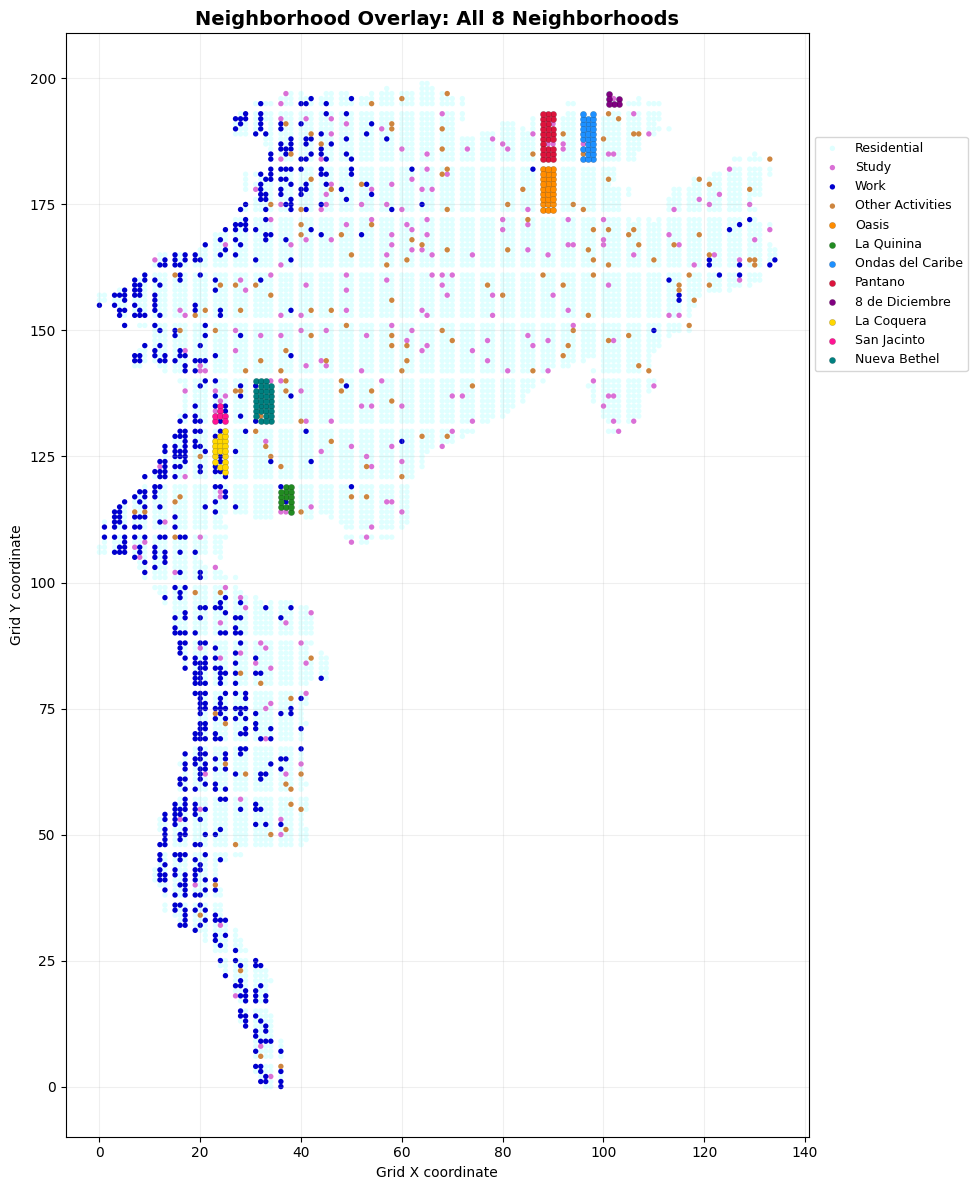
\includegraphics[width=0.85\textwidth]{Images/map_neighborhoods.png}
\caption{Spatial distribution of residential cells by neighborhood on the model grid. Colors distinguish the eight sentinel localities (Oasis, La~Quinina, Ondas del~Caribe, Pantano, 8~de~Diciembre, La~Coquera, San~Jacinto, and Nueva~Bethel) against the background of non-residential active cells. Grid axes are in cell units ($x$: 0--140, $y$: 0--205).}
\label{fig:neighborhoods}
\end{figure}

\begin{table}[h]
\centering
\caption{Target and realized cell counts by sentinel neighborhood. Shortfall equals target minus realized; proportion equals realized divided by target.}
\label{table:neighborhood_coverage}
\begin{tabular}{clcccc}
\toprule
\textbf{ID} & \textbf{Neighborhood} & \textbf{Target} & \textbf{Realized} & \textbf{Shortfall} & \textbf{Proportion} \\
\midrule
1 & Oasis            & 108 &  37 &  71 & 0.343 \\
2 & La Quinina       & 172 &  19 & 153 & 0.110 \\
3 & Ondas del Caribe & 100 &  27 &  73 & 0.270 \\
4 & Pantano          & 103 &  26 &  77 & 0.252 \\
5 & 8 de Diciembre   & 147 &   7 & 140 & 0.048 \\
6 & La Coquera       & 147 &   9 & 138 & 0.061 \\
7 & San Jacinto      & 147 &  21 & 126 & 0.143 \\
8 & Nueva Bethel     & 122 &  31 &  91 & 0.254 \\
\bottomrule
\end{tabular}
\end{table}

Across all neighborhoods, the total target was 1{,}046 cells and the realized allocation was 177 cells, corresponding to a global realized proportion of 0.169. The largest shortfalls occurred in La~Quinina, 8~de~Diciembre, and La~Coquera. These neighborhoods are located in or adjacent to the coastal fringe, where tourist and commercial land uses dominate and residential cells are comparatively scarce. The algorithm terminated early in these zones when the local supply of contiguous residential cells was exhausted, which is consistent with the city's documented mixed land-use structure rather than a methodological artifact. The two neighborhoods with the highest realized counts were Oasis (37 cells) and Nueva~Bethel (31 cells), both located further inland with more continuous residential cells. Because these clusters serve to localize vector heterogeneity rather than to produce neighborhood-level incidence estimates, the reduced cell counts simply concentrate the HI activation within the most residential cores and leave the citywide calibration and validation unaffected.

\subsection{HI-informed mosquito emergence}
\label{sec:results_hi}

Table~\ref{table:hi_activation} reports the neighborhood-level summary of the stochastic activation driven by the House Index. For most neighborhoods, the realized activation rate exceeded the nominal HI by a positive margin, which is consistent with sampling variability from Bernoulli draws over small populations of residential cells. The magnitude of the deviation scaled inversely with the number of cells available in each neighborhood. For example, 8~de~Diciembre, with only seven cells, showed a deviation of 0.246, while Oasis, with 37~cells, showed a deviation of 0.075.

\begin{table}[H]
\centering
\caption{HI-based stochastic activation by neighborhood. HI is the neighborhood mean House Index used as the Bernoulli activation probability. Realized AR is the proportion of cells with $X_i = 1$. Diff = Realized AR $-$ HI.}
\label{table:hi_activation}
\begin{tabular}{clcccc}
\toprule
\textbf{ID} & \textbf{Neighborhood} & \textbf{Cells} & \textbf{HI} & \textbf{Realized AR} & \textbf{Diff} \\
\midrule
1 & Oasis            & 37 & 0.249 & 0.324 & $+$0.075 \\
2 & La Quinina       & 19 & 0.217 & 0.263 & $+$0.046 \\
3 & Ondas del Caribe & 27 & 0.287 & 0.407 & $+$0.121 \\
4 & Pantano          & 26 & 0.257 & 0.423 & $+$0.167 \\
5 & 8 de Diciembre   &  7 & 0.325 & 0.571 & $+$0.246 \\
6 & La Coquera       &  9 & 0.275 & 0.333 & $+$0.058 \\
7 & San Jacinto      & 21 & 0.259 & 0.476 & $+$0.217 \\
8 & Nueva Bethel     & 31 & 0.271 & 0.258 & $-$0.013 \\
\bottomrule
\end{tabular}
\end{table}

Figure~\ref{fig:hi_activation} shows the spatial footprint of activated residential cells ($X_i = 1$) across the model grid. Activation was concentrated within the eight delineated neighborhoods, leaving residential areas elsewhere at the baseline floor~$\eta$.

\begin{figure}[ht]
\centering
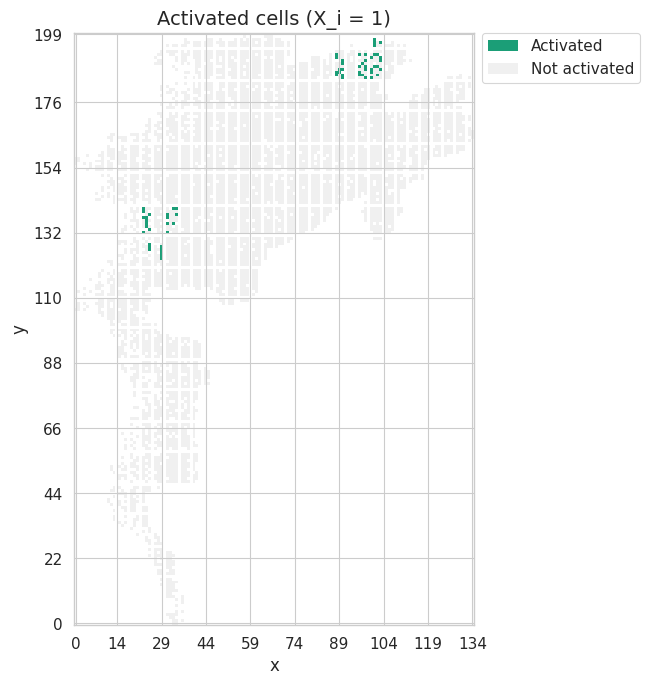
\includegraphics[width=0.85\textwidth]{Images/activated_cells.png}
\caption{Activated residential cells ($X_i = 1$) under HI-based stochastic allocation. Activated cells are shown in teal; non-activated residential cells are shown in gray. The map highlights the spatial heterogeneity in adult mosquito recruitment introduced by the House Index.}
\label{fig:hi_activation}
\end{figure}

\subsection{Reported and adjusted citywide incidence}
\label{sec:results_incidence}

Figure~\ref{fig:incidence_adj} shows the reported and adjusted incidence trajectories over the full 2023--2024 record. The expansion factor shifted the series upward uniformly, with peak adjusted incidence reaching approximately 68 cases per 100{,}000 late in 2023, compared to a peak reported incidence of approximately 9 per 100{,}000 in the same week. Crucially, the adjustment preserved the temporal structure of the series, since the timing of local maxima and minima coincided across both curves. This alignment supported the use of the adjusted series as the calibration target, since the goal was to match the temporal profile of transmission while correcting for systematic under-counting.

\begin{figure}[H]
\centering
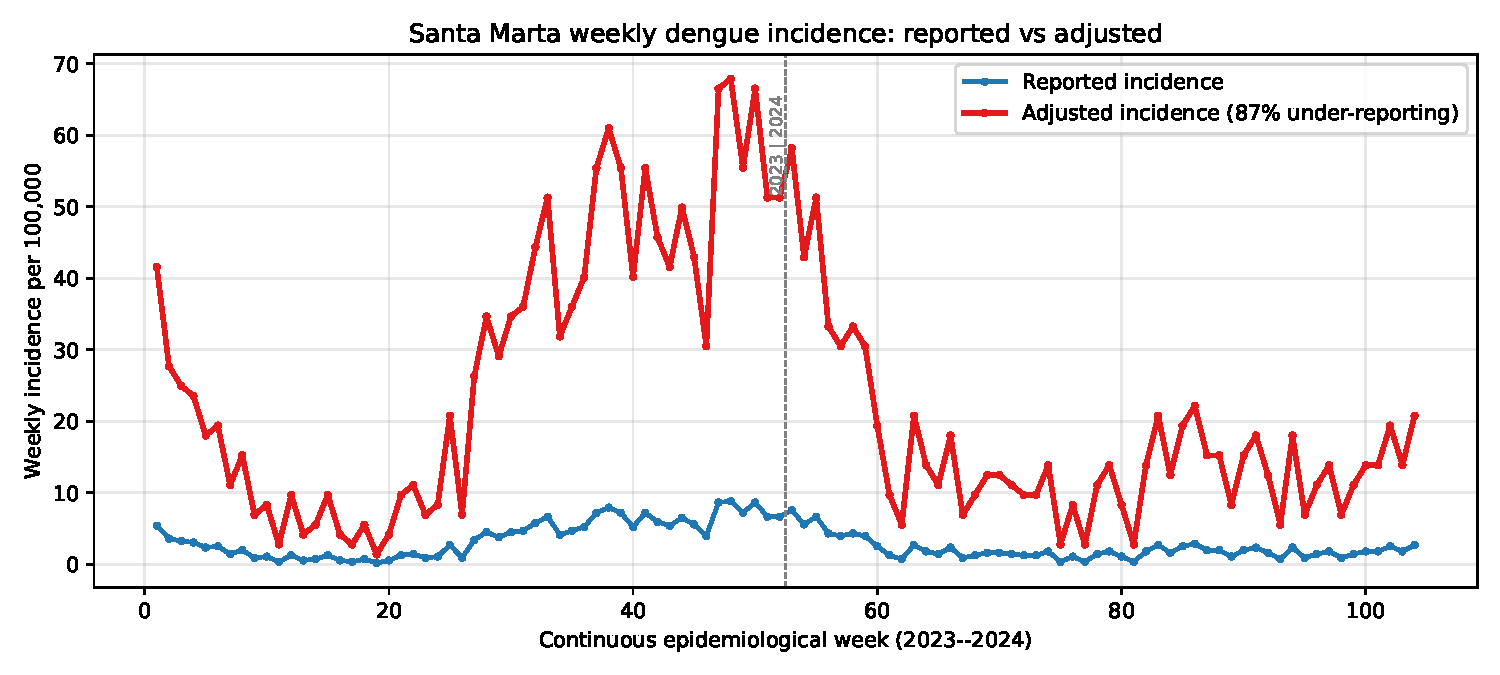
\includegraphics[width=0.85\textwidth]{Images/incidence_reported_adjusted.pdf}
\caption{Santa Marta weekly dengue incidence per 100{,}000 inhabitants: reported (blue) and adjusted with expansion factor $\rho = 0.13$ (red), over the full 2023--2024 record. No smoothing applied.}
\label{fig:incidence_adj}
\end{figure}

\subsection{Calibration results}
\label{sec:results_calibration}

The search converged to an operating point with a small initial seed of $\hat{I}_0 = 2$, a small interaction exponent of $\hat{z} = 0.05$, and a transmission intensity of $\hat\beta = 0.32$. At this point the simulated epidemic reproduced the early dynamics of the adjusted surveillance series, with the simulated and observed peaks of the same height and in the same week. The simulated annual attack rate was about $0.7$ per~100 inhabitants, of the same order as the adjusted observed rate of about $1.2$ per~100 over the selected window. We note that $\hat{z}$ and $\hat\beta$ lie at the edges of their search ranges. The objective keeps improving toward lower $z$ and higher $\beta$, with no interior optimum, which indicates that these transmission parameters are weakly identified from a single season of citywide incidence. Figure~\ref{fig:identifiability} shows this directly, as the composite objective across the evaluated candidates decreases toward the lower bound of $z$ and the upper bound of $\beta$, and the selected point sits at that corner. We return to this point in Section~\ref{sec:discussion}.

\begin{figure}[H]
\centering
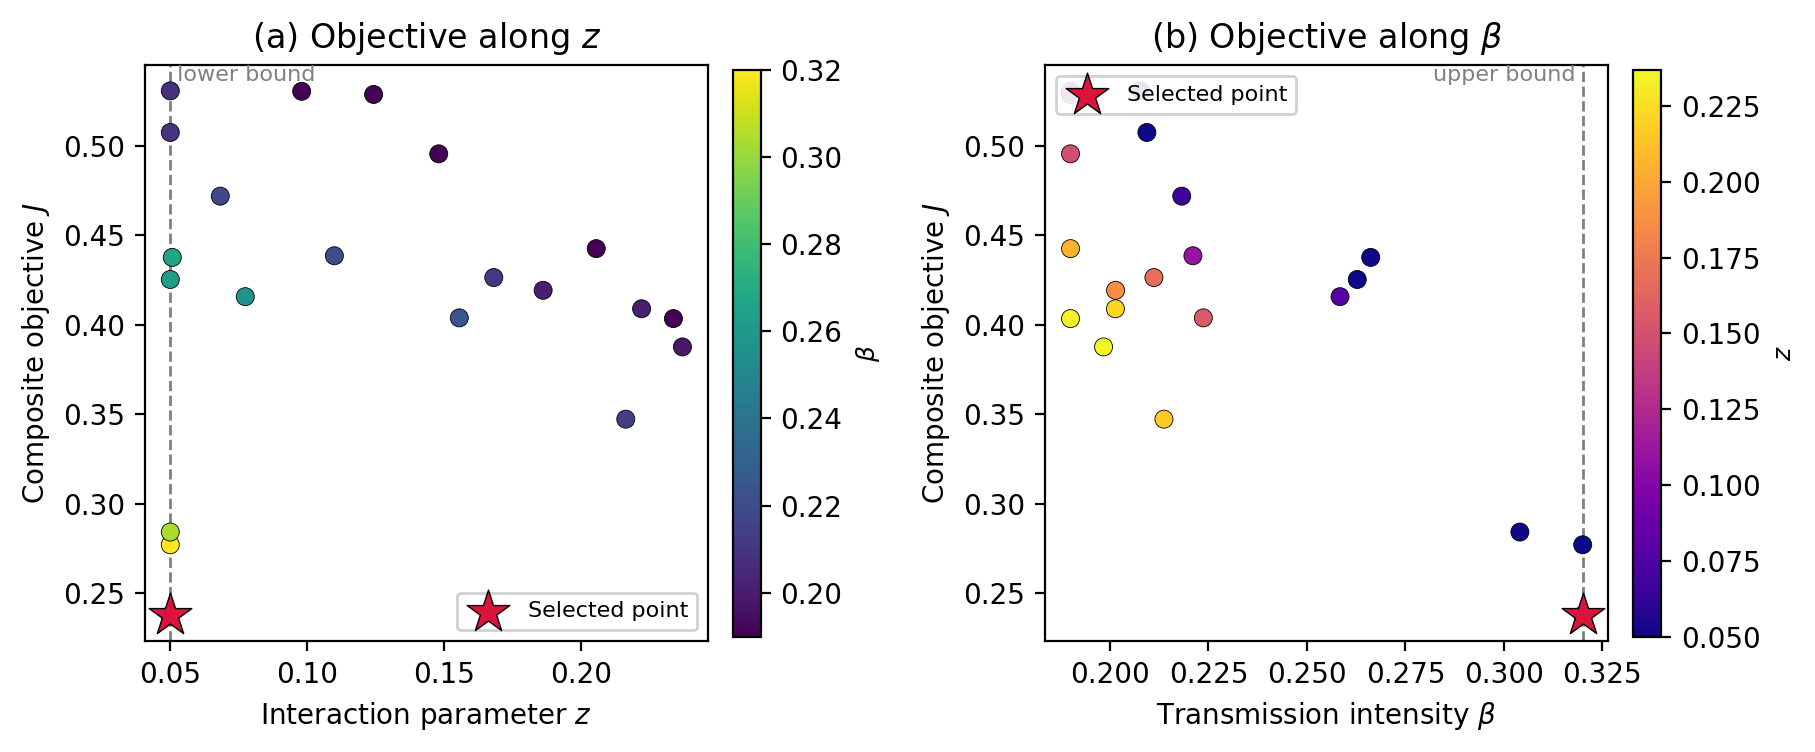
\includegraphics[width=0.95\textwidth]{Images/identifiability.png}
\caption{Composite objective $J$ across the Bayesian-optimization candidates, evaluated along the interaction parameter $z$ in panel~(\textbf{a}) and the transmission intensity $\beta$ in panel~(\textbf{b}), where lower values are better. Marker colour encodes the complementary parameter. The objective decreases toward the lower bound of $z$ and the upper bound of $\beta$, with no interior minimum, and the selected operating point (red star) lies at that corner. This boundary behaviour shows that $z$ and $\beta$ are weakly identified from a single season of citywide incidence.}
\label{fig:identifiability}
\end{figure}

The best-matching observed window begins at week~45 of 2023, near the seasonal peak, and runs into 2024. Figure~\ref{fig:calibration_bands} shows the comparison over that window, with the median trajectory and the 70\% prediction band. The figure reports the median rather than the mean, because the replicates are skewed near the epidemic threshold; a few take off early and inflate the mean, so the median tracks the typical seasonal wave more faithfully. The simulated median followed the observed peak and its decline very closely, and the similarity metrics are reported in Section~\ref{sec:results_validation}. The agreement is strongest over the first fifteen weeks, which contain the peak and the main decline. After that the simulated median falls to zero, while the observed series keeps a small but persistent tail, so the band encloses about half of the observed weeks. We examine the wide early band and the missing tail in Section~\ref{sec:discussion}.

\begin{figure}[H]
\centering
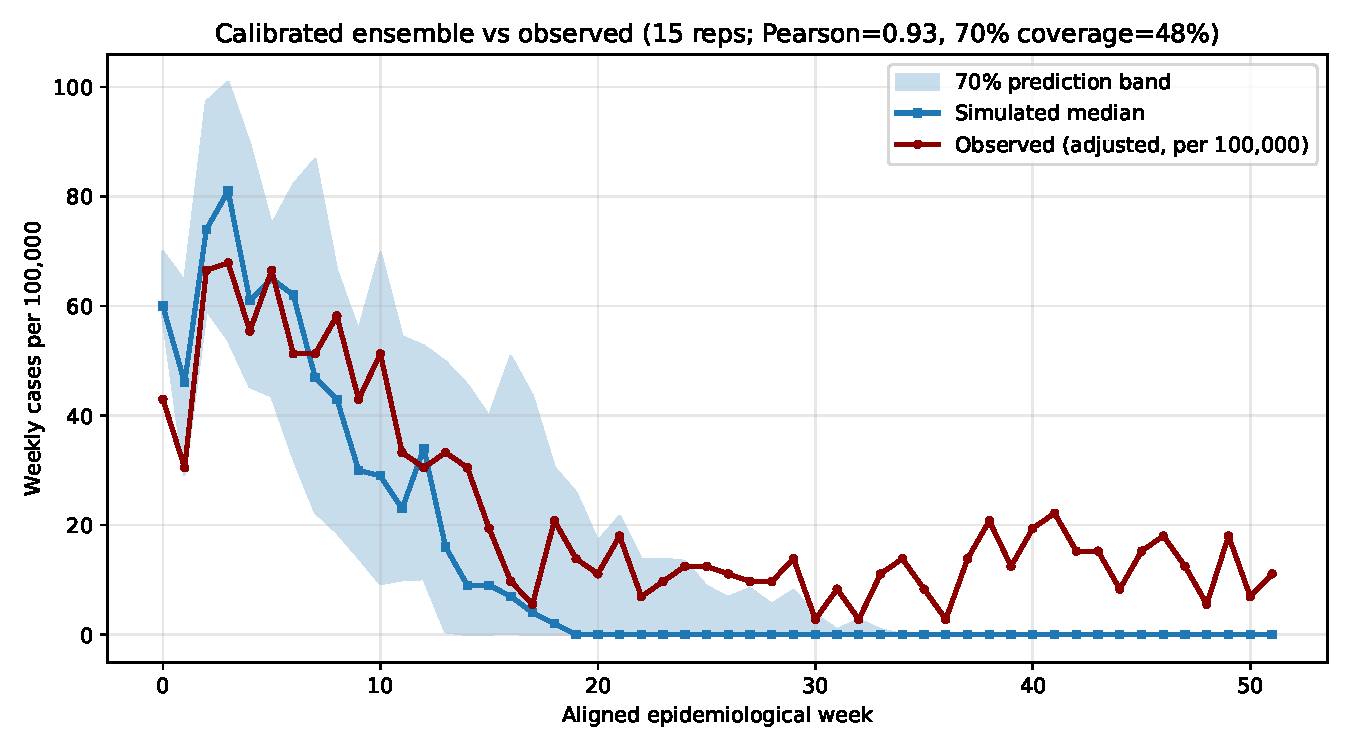
\includegraphics[width=0.85\textwidth]{Images/calibration_fit.pdf}
\caption{Calibrated simulation with 15 replicates. Blue line: median simulated weekly cases per 100{,}000; shaded band: 70\% prediction interval (15th--85th percentile across replicates); dark-red line: observed adjusted weekly incidence from the best-matching 52-week window of the 2023--2024 record. Axes: aligned epidemiological week and weekly cases per 100{,}000.}
\label{fig:calibration_bands}
\end{figure}

\subsection{Validation results}
\label{sec:results_validation}

\subsubsection{Shape comparison and temporal correlation}

Figure~\ref{fig:shape_comparison} shows the z-standardized and smoothed weekly incidence series for the simulated median and the observed surveillance data. The two series shared a common overall waveform, with a high period in the first half of the alignment window and a lower period thereafter.

\begin{figure}[H]
\centering
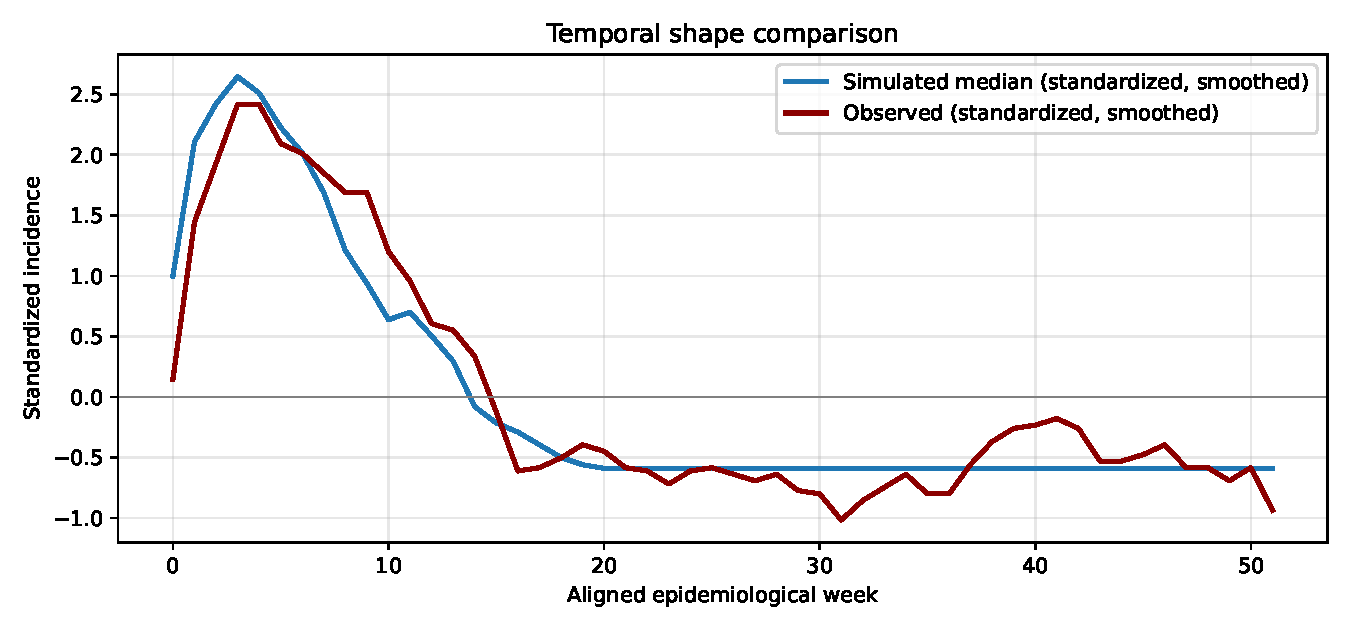
\includegraphics[width=0.85\textwidth]{Images/shape_comparison.pdf}
\caption{Shape comparison between simulated weekly cases (median across replicates, smoothed with a centered three-week rolling mean and z-standardized) and observed weekly incidence (smoothed and z-standardized). Vertical axis: z-scores; horizontal axis: aligned epidemiological week.}
\label{fig:shape_comparison}
\end{figure}

The statistical similarity metrics are reported in Table~\ref{table:validation_metrics}. At zero lag, the Pearson correlation was 0.93 and the Spearman rank correlation was 0.75, indicating strong linear and monotonic agreement in standardized amplitudes. After standardizing and smoothing both series, the Pearson correlation rose to 0.96. Because the comparison window was already aligned during calibration, the best additional lag was zero weeks. Directional agreement, the proportion of consecutive weekly changes in the same direction, was 29\%. The model thus reproduced the broad seasonal pattern faithfully, while the fine fluctuations from one week to the next remain a target for further refinement.

\begin{table}[H]
\centering
\caption{Similarity metrics between the simulated median and the observed adjusted incidence over the selected window, for 15 replicates at the calibrated point. Shape correlations are computed after standardizing and smoothing both series.}
\label{table:validation_metrics}
\begin{tabular}{lcc}
\toprule
\textbf{Metric} & \textbf{Value} & \textbf{Units} \\
\midrule
Pearson correlation, raw (lag 0)   & 0.93 & -- \\
Pearson correlation, shape (lag 0) & 0.96 & -- \\
Spearman correlation (lag 0)       & 0.75 & -- \\
Best additional lag (Pearson)      & 0    & weeks \\
RMSE of the standardized series    & 0.29 & SD units \\
70\% prediction-band coverage      & 48   & \% \\
Directional agreement              & 29   & \% \\
\bottomrule
\end{tabular}
\end{table}

\subsubsection{Prediction-band coverage}

With the transmission intensity calibrated, the simulated and observed series are of comparable magnitude over the peak. The 70\% prediction band in Figure~\ref{fig:calibration_bands} covers the observed trajectory closely over the peak and the main decline. Coverage over the whole window is about half of the observed weeks. The remaining differences are concentrated in the low tail of the season, where the observed series keeps a small but persistent level while the simulated median has already fallen to zero. The closed-population model does not hold this tail once the early seeding impulse has decayed. We return to this point in Section~\ref{sec:discussion}.

\subsubsection{Expert review}

Conceptual validation was conducted with Dr.~Gabriel Parra Henao, an epidemiologist from the Secretary of Health of Medellín with extensive field experience in dengue surveillance in Colombia. Table~\ref{table:expert_review} summarizes the structured assessment.

\begin{table}[H]
\centering
\caption{Expert review by Dr.~Gabriel Parra Henao. Comments are paraphrased from the structured review session.}
\label{table:expert_review}
\begin{tabularx}{\textwidth}{>{\bfseries}p{3.5cm} X}
\toprule
Aspect & Expert assessment \\
\midrule
Face validity & The simulated dynamics were considered consistent with known dengue transmission patterns, despite the higher magnitude relative to reported incidence. \\
Parameter plausibility & The nominal parameter values were endorsed as reasonable approximations with realistic magnitudes, acknowledging uncertainty in precise values. \\
Perceived utility & The model was considered to have potential utility for comparative analysis of transmission scenarios. \\
Operational metric & In practice, field evaluation of control strategies relies on Aedes indices rather than case counts. Obtaining such indices requires field measurements not available at the citywide scale in the current data. \\
Model perspective & The model's primary value was identified as its capacity to represent transmission dynamics from the human behavioral perspective, complementing mosquito-focused approaches. \\
\bottomrule
\end{tabularx}
\end{table}

\subsubsection{Sensitivity analysis}
\label{sec:results_sa}

Figure~\ref{fig:nsc} and Table~\ref{table:sensitivity} report the normalized sensitivity coefficients for a $+10\%$ change in each of the seven parameters. These coefficients are measured in the super-critical reference regime, where the epidemic reliably takes off and reaches an attack rate near $94\%$ (Table~\ref{table:sensitivity}). The peak magnitudes there are accordingly about two orders of magnitude above the fitted citywide peak of roughly $68$ per $100{,}000$, so the analysis reports the leverage and ranking of each parameter rather than magnitudes comparable to the calibrated season. The transmission couplings dominate. The human-to-mosquito probability $\beta_{hm}$ was the most influential parameter, with a coefficient of $4.32$. The patch carrying capacity $C$ followed at $3.40$, then the interaction parameter $z$ at $2.94$, and the mosquito-to-human probability $\beta_{mh}$ at $2.45$. The mosquito reproduction rate $r$ was weaker at $1.27$. The bite-availability parameters were weakest, at $1.01$ for $\sigma_H$ and $0.50$ for $\sigma_M$. A rise in any transmission parameter raised the epidemic peak and also moved it earlier, from week~17 toward week~12. This pattern is expected, because these parameters jointly set the effective reproduction number of the coupled human--vector system.

\begin{figure}[H]
\centering
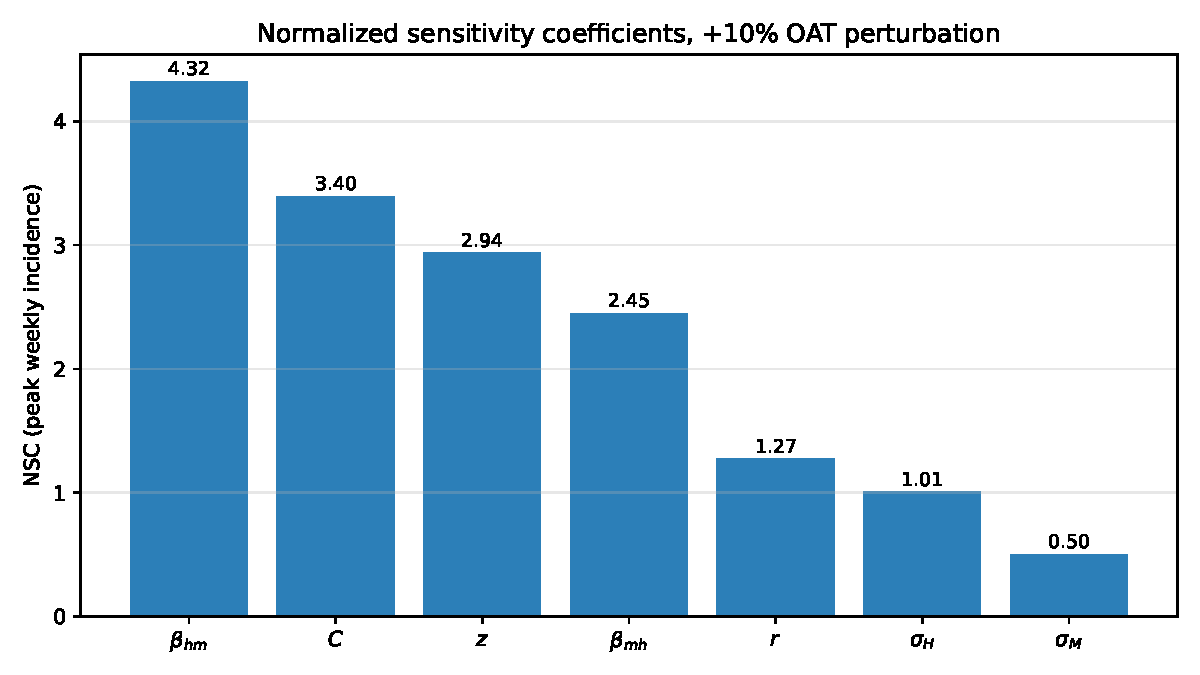
\includegraphics[width=0.7\textwidth]{Images/nsc_7param.pdf}
\caption{Normalized sensitivity coefficients (NSC) for a $+10\%$ change in each parameter, measured as the proportional change in median peak weekly incidence in Equation~\eqref{eq:nsc_peak}.}
\label{fig:nsc}
\end{figure}

\begin{table}[H]
\centering
\caption{Seven-parameter one-at-a-time sensitivity analysis, evaluated in the super-critical reference regime ($\beta=0.35$, $z=0.118$). The peak $p$ is the median peak weekly incidence in cases per 100{,}000 and the peak week is read from the same trajectory, at the reference point and under each $+10\%$ change. The attack rate is the seasonal fraction of the population that becomes infected. The coefficient follows Equation~\eqref{eq:nsc_peak}.}
\label{table:sensitivity}
\begin{tabular}{lcccc}
\toprule
\textbf{Parameter} & \textbf{Peak} $p$ & \textbf{Peak week} & \textbf{Attack rate (\%)} & \textbf{NSC} \\
\midrule
Reference              & 14520 & 17 & 94.3 & --   \\
$\beta_{hm}$ ($+10\%$) & 20799 & 12 & 98.2 & 4.32 \\
$C$ ($+10\%$)          & 19449 & 13 & 98.2 & 3.40 \\
$z$ ($+10\%$)          & 18785 & 14 & 97.8 & 2.94 \\
$\beta_{mh}$ ($+10\%$) & 18077 & 15 & 97.5 & 2.45 \\
$r$ ($+10\%$)          & 16367 & 15 & 96.1 & 1.27 \\
$\sigma_H$ ($+10\%$)   & 15982 & 15 & 96.1 & 1.01 \\
$\sigma_M$ ($+10\%$)   & 15248 & 16 & 96.2 & 0.50 \\
\bottomrule
\end{tabular}
\end{table}

\section{Discussion}
\label{sec:discussion}

This study presented an end-to-end workflow for adapting and validating a hybrid agent-based model of dengue transmission in a specific urban setting. The workflow integrated geospatial adaptation, expert-informed biological parameterization, high-performance execution, simulation-based calibration, and pattern-oriented validation into a single reproducible process. The Santa Marta case study demonstrated both the potential and the current limitations of this approach.

\subsection{Spatial adaptation and neighborhood delineation}

The GIS-based spatial adaptation translated the abstract grid topology of the Bello prototype into a city-specific representation grounded in real land-use data. The BFS flood-fill procedure successfully delineated all eight sentinel neighborhoods, though the realized residential cell coverage was lower than the nominal targets in several localities (global proportion of 0.169). This outcome was expected, because the algorithm restricted growth to residential cells, and neighborhoods in Santa Marta's coastal and tourist zones contain a high density of commercial and leisure land uses that reduced the contiguous residential supply. The coverage pattern therefore reflected the city's actual land-use heterogeneity rather than a failure of the delineation method. In this study the clusters act as a device for localizing HI-informed vector heterogeneity rather than as units of neighborhood-level epidemiological inference, so the reduced counts leave the citywide calibration and validation unaffected. Future work could broaden their role by allowing neighborhoods to include non-residential cells with a reduced weight, or by refining the OSM land-use classification with local cartographic data.

\subsection{HI-informed emergence and spatial heterogeneity}

The stochastic activation mechanism linked patch-level mosquito emergence to the House Index measured in each neighborhood, introducing spatial heterogeneity in vector recruitment that matched observed entomological conditions at the neighborhood scale. The realized activation rates generally tracked the nominal HI values, with deviations explainable by binomial sampling variability over small cell populations. The mechanism improved the spatial realism of mosquito density in the intervention areas without altering the intrinsic demographic parameters $r$ and $C$, maintaining interpretability. A limitation of the current implementation is that the HI-based mask was fixed at initialization and treated as stationary, ignoring seasonal variation in breeding conditions and potential spatial clustering of productive sites. Incorporating time-varying or spatially correlated activation would be a natural extension.

\subsection{Calibration and identifiability}

The calibration and the sensitivity analysis are the quantitative core of the workflow that this study sets out to demonstrate, the adaptation of an established hybrid agent-based model to a new city. High-performance execution made this core practical. The surrogate search and the sensitivity runs together required more than one hundred year-long runs, which the parallel scheme of Section~\ref{sec:implementation} reduced to a single overnight run on one multi-core workstation. The findings below should be read in that light, as lessons about adapting the model to a new setting rather than as facts about Santa Marta alone.

The calibration estimated the transmission intensity together with the initial seed and the interaction exponent, and it placed the simulated season at the right magnitude. The resulting operating point sits close to the model's epidemic threshold, which is the point at which the reproduction number equals one. The reproduction number is the average number of further infections caused by one infected case. When it is below one an outbreak dies out, and when it is above one an outbreak grows. The Santa Marta season has a small attack rate, near $1$ per~100 after adjustment. A closed-population model reaches so small an attack rate only when its reproduction number is just above one, so the calibrated operating point sits just above the threshold. This position explains the width of the prediction band. So close to the threshold the epidemic only barely takes off, and whether it takes off early or late is largely a matter of chance. Individual replicates therefore peak in different weeks, and the resulting prediction band is wide, even though each replicate is internally consistent.

The proximity to the threshold also limits identifiability. Several transmission parameters, namely $\beta_{mh}$, $\beta_{hm}$, and $z$, act through the same reproduction number. They are therefore hard to separate from a single season of citywide incidence. The calibration result shows this directly. The estimated $z$ and $\beta$ settle at the edges of their search ranges, because the objective keeps improving toward lower $z$ and higher $\beta$ without a clear interior optimum (Figure~\ref{fig:identifiability}). The sensitivity analysis measures the individual leverage of these parameters, but it does not resolve their overlap. Richer targets would be needed to identify the transmission parameters one by one. Useful targets include several seasons, incidence stratified by age or neighborhood, and entomological indices. This limit is not specific to Santa Marta. Any city to which the model is adapted will face it, because a single season of citywide incidence pins down the overall transmission scale but not the individual parameters. The workflow is useful here precisely because it makes that boundary visible, and it shows where additional local data would most improve a future adaptation.

\subsection{Decline of the simulated season and the missing tail}

The simulated season rises to a peak and then declines toward zero before the observed season ends. The root cause of this decline lies on the vector side of the transmission cycle, in the dynamics of the infected mosquito population. At the calibrated point only about one person in one hundred and forty is ever infected, so the human susceptible pool stays almost full throughout the season and the season instead ends through the vector dynamics described below.

The early wave is driven mainly by the initial conditions. At the start of the run there are a few infected humans, and each patch holds a small number of infected mosquitoes set at initialization. Together these produce the rapid rise and the peak. For the epidemic to continue beyond this initial impulse, the transmission cycle must turn on its own. Infected humans must infect mosquitoes, and those mosquitoes must in turn infect more humans. The strength of the first step, from human to mosquito, is governed by the interaction parameter $z$ through $\Psi_h$.

Calibration drove $z$ to a low value. A low $z$ makes the human-to-mosquito step weak, so infected humans generate few new infected mosquitoes. At the same time, adult mosquitoes are short-lived, so the infected mosquitoes present at the start are steadily removed by mortality. When the weak feedback cannot replace them as fast as they die, the infected-mosquito population falls toward zero. Once a patch has no infected mosquitoes left, there is no longer any route to infect the humans there, and local transmission stops. The model has no mechanism to reintroduce infection, so the stop is permanent. This is why the simulated curve reaches zero around week nineteen and stays there.

The same reasoning explains why the model cannot hold the long low tail of the observed season. The observed series keeps a small but persistent level of cases through the rest of the year. In a real city this persistence is maintained by processes that lie outside the closed model. Infected travellers keep arriving in a tourism hub such as Santa Marta, infection is reintroduced between neighborhoods, and the susceptible pool is slowly replenished. The model has none of these. With a closed population and a weak internal feedback, the simulated epidemic is in effect a single pulse seeded at the start. Once that pulse decays, nothing remains to sustain transmission. These reintroduction and seasonal mechanisms take a particular form in Santa Marta, where climate, household water storage, population concentration, and tourism-related mobility interact across the year to shape when and where transmission persists \cite{MARTIN2026100164}. The missing tail therefore reflects a city specific gap in the closed model rather than a generic absence of external seeding.

This also clarifies the role of the calibration in the decline. The optimizer favored a low $z$ because a weak, fast-decaying wave produces the sharp peak that best matches the observed peak in shape. A higher $z$ would let the cycle sustain itself longer and would fill in more of the tail, but it would also broaden and lower the peak and reduce the shape correlation. The calibration therefore traded the tail for the peak. The missing tail is thus partly a structural property of the closed model and partly a consequence of the operating point that the shape-based objective selected.

\subsection{Validation and temporal agreement}

The validation results provided convergent evidence that the model captured the seasonal structure of dengue transmission in Santa Marta. The Pearson and Spearman correlations at zero lag, $0.93$ and $0.75$, together with the shape correlation of $0.96$, indicated strong agreement in the temporal pattern of rises and falls, even though week-to-week directional agreement was limited at $29\%$. Because the comparison window was aligned during calibration, no residual phase offset remained. The agreement is strongest over the peak and the main decline, while the late low tail is not reproduced, for the reasons given above.

The expert review endorsed the model's face validity and parameter plausibility while highlighting a practical consideration. Field evaluation of vector control strategies in Colombia relies on Aedes indices (House, Container, and Breteau indices) rather than case counts. Because the current model does not produce these indices directly, comparisons of simulated control scenarios with real-world interventions assessed by entomological field teams cannot be performed without an additional mapping module. This represents a clear direction for future development.

\subsection{Limitations and future directions}

Several aspects also point to clear opportunities for refinement. First, the calibrated point sits near the epidemic threshold, where random take-off widens the prediction band. Narrowing the band would call for either tighter constraints in the objective or a mechanism that makes the timing of the epidemic take-off more consistent across replicates. Second, as explained above, the model uses a closed population with permanent immunity and no external introductions or demographic turnover, so it produces a single seasonal wave and concentrates its agreement over the peak and the main decline. For a tourism hub such as Santa Marta, adding external introductions of infection is the most direct next step. A small and continuous external force of infection would supply the low tail and would also make the timing of the take-off steadier. Third, the synthetic population was scaled down to keep runtime manageable and compared with the observed series on a per-100{,}000 basis. Because vector pressure scales with the mosquito-to-human ratio, absolute counts should be read at the calibrated scale and not transferred across population sizes. Fourth, the HI data originated from inspected subsets of dwellings and may carry selection and measurement biases that propagate to the emergence multipliers, and the HI-based mask was fixed at initialization and treated as stationary, which leaves seasonal change in breeding conditions as a further extension. A natural extension is to replace this stationary mask with richer, time-varying environmental layers, such as NDVI, NDWI, precipitation, and seasonal climate patterns, so that mosquito recruitment and breeding site suitability vary across space and time and stay closer to locally observed conditions in Santa Marta. Driving these layers with their observed timing would also let the model carry the delayed environmental effects, at lags of one to four weeks, that the local evidence links to dengue incidence in the city \cite{MARTIN2026100164}.

Future work will follow three priorities. The first is to add external introductions of infection, and optionally seasonal forcing of vector abundance, so the model can sustain a low tail and stand away from the bare threshold. The second is an entomological output module that computes Aedes indices from the simulated state, which would allow comparison with the field metrics used to evaluate control in Colombia. The third is the analysis of control strategies, such as pulse vaccination and pyriproxyfen larval control, on the calibrated and validated baseline. Each of these extensions serves the central aim of this study, which is a model that adapts across cities and climates and supports the comparison of control strategies. The calibration and sensitivity workflow shown here, together with its high-performance backbone, is the part that makes such adaptation repeatable in a new setting, rather than a result tuned to one dataset.

\section{Conclusions}
\label{sec:conclusions}

This paper presented an end-to-end workflow for adapting a hybrid agent-based model of dengue transmission in a specific urban setting, demonstrated through a case study in Santa Marta, Colombia. Building on prior development work for Bello~\cite{escudero2023hybrid,uribe2023ccc}, the workflow integrated GIS-based spatial adaptation, HI-informed mosquito emergence, high-performance execution in Repast HPC, surrogate-based multi-parameter calibration, and pattern-oriented validation against weekly surveillance data.

The main findings were as follows. The BFS neighborhood delineation successfully identified eight sentinel localities, with coverage patterns reflecting the city's coastal land-use structure rather than methodological limitations. The HI-informed emergence allocation introduced spatially heterogeneous vector recruitment consistent with observed entomological conditions at the neighborhood scale. The multi-parameter calibration placed the simulated season at the right magnitude and reproduced the peak and the main decline of the adjusted surveillance series (Pearson $r = 0.93$ at lag 0; shape correlation $0.96$). The calibrated operating point sits near the epidemic threshold, where the transmission parameters are only weakly identified from a single season, and the closed-population structure does not sustain the late low tail. These findings mark external introductions of infection, seasonal forcing, and richer calibration targets as the priorities for refinement.

The workflow is designed to be transferable. Any city for which a GeoJSON urban mask and a CSV temperature series are available can be configured as a new case study by updating the city-specific inputs in Stages~3 through~5 while reusing the model architecture and the HPC scaffolding. This modularity supports the broader goal of building a reproducible workflow toward adaptable, locally validated decision support for dengue control in Colombian cities.

\authorcontributions{Conceptualization, P.E. and L.L.; methodology, L.L., S.M.C. and P.E.; software, L.L. and S.M.C.; calibration and validation, S.M.C.; expert epidemiological validation and support, G.P.; formal analysis, S.M.C. and L.L.; investigation, L.L. and S.M.C.; writing of the original draft, L.L., S.M.C. and P.E.; review and editing, P.E., S.M.C. and G.P.; visualization, S.M.C. and L.L.; supervision, P.E.; project administration, P.E.; funding acquisition, P.E. All authors have read and agreed to the published version of the manuscript.}

\funding{This research was funded by Universidad EAFIT, Medellín, Colombia. The funding was provided through a research grant led by Professor Paula Escudero. The grant supported Luisa F. Londoño master's degree studies, covering tuition fees and maintenance for a duration of two years.}

\institutionalreview{Not applicable}

\informedconsent{Not applicable as this article does not involve any human participants.}

\dataavailability{The surveillance datasets presented in this article are not readily available because they are part of an ongoing study, and requests to access them should be directed to the authors. The model source code, the synthetic-population generator, and the calibration and sensitivity-analysis scripts are openly available at \url{https://github.com/smcanom/dengue-habm-santamarta}.}

\acknowledgments{The authors wish to acknowledge to Universidad EAFIT for the provision of computational facilities and specially to Maria Eugenia Puerta Yepes, Juan Pablo Ramirez Ramirez, Harold Steven Gonzalez Ossa, Alexandra Cataño Lopez and Daniel Rojas Diaz for all their valuable insights and support to this research.}

\conflictsofinterest{The authors declare no conflicts of interest. The funding received by Luisa F. Londoño does not lead to any conflict of interest regarding the publication of this study.} 

\abbreviations{Abbreviations}{
The following abbreviations are used in this manuscript:\\

\noindent 
\begin{tabular}{@{}ll}
ABMS & Agent-based Modeling and Simulation\\
HABMS & Hybrid Agent-based Modeling and Simulation\\
HPC & High-Performance Computing\\
ODE & Ordinary Differential Equations
\end{tabular}
}

\begin{adjustwidth}{-\extralength}{0cm}

\reftitle{References}

\bibliography{references.bib}

\PublishersNote{}
\end{adjustwidth}
\end{document}